%preamble - package inclusion and set up
\documentclass[12pt,twoside,a4paper,english]{report} %normalt 12pt!!!!
% Select encoding of your inputs
\usepackage[utf8]{inputenc}
% Make latex understand and use the typographic
% rules of the language used in the document.
%\usepackage[danish]{babel}
\usepackage[english]{babel}

% Use the vector font Latin Modern which is going
% to be the default font in latex in the future.
%\usepackage{lmodern}
\usepackage{mathptmx}

% Choose the font encoding
\usepackage[T1]{fontenc}

% Use color in tables
\usepackage[table]{xcolor}
\usepackage{pbox}
\usepackage{tabularx}
\usepackage{array}
\usepackage{multirow}

% Load a colour package
\usepackage{xcolor}
\definecolor{aaublue}{RGB}{33,26,82}  %<--define aaublue
\definecolor{white}{RGB}{255,255,255} %<--define white

% ref stuffz			original position
%\usepackage{cleveref}

% The standard graphics inclusion package
\usepackage{graphicx}

\makeatletter
  \g@addto@macro\@floatboxreset\centering %<--centering all figures
\makeatother

\usepackage{adjustbox}

% Set up how figure and table captions are displayed

\usepackage{float}
\restylefloat{figure}
\usepackage{caption}
\usepackage{subfigure}
\usepackage[subfigure]{tocloft}
\captionsetup
{
  %justification = centering,    %<--centering caption with multiple lines
  %justification = raggedright,  %<-- right alings caption with multiple lines
  justification = justified,  %<-- justify alings (make left and right side equal) caption with multiple lines
  font          = footnotesize, %<--set font size to footnotesize
  labelfont     = bf            %<--bold label (e.g., Figure 3.2) font
}
\captionsetup[subfigure]
{
  justification = centering, %<--centering subfigure caption text
  singlelinecheck=false,
  font = footnotesize        %<--font size for subfigures
} 

% Enable row combination in tables
\usepackage{multirow}

% Make space between table lines and text
\renewcommand{\arraystretch}{1.5}

% Enable commands like \st (strike out) and \hl (high light)
\usepackage{soul}

% Make the standard latex tables look so much better
\usepackage{array,booktabs}

% Enable the use of frames around, e.g., theorems
% The framed package is used in the example environment
\usepackage{framed}
\usepackage{colortbl}
\usepackage{longtable}
\usepackage{xcolor}
\usepackage{textcomp}

%-------MATHEMATICS---------------------------------
% Defines new environments such as equation,
% align and split 
\usepackage{amsmath}
\usepackage{relsize}
% Adds new math symbols
\usepackage{amssymb}
% Use theorems in your document
% The ntheorem package is also used for the example environment
% When using thmmarks, amsmath must be an option as well. Otherwise \eqref doesn't work anymore.
\usepackage[framed,amsmath,thmmarks]{ntheorem}
\usepackage{xifthen}%<--enables ifthenelse which is used in macros

\usepackage{siunitx} 
\sisetup{decimalsymbol=period}%<--\num{} will swich commas with periods
\sisetup{detect-weight}
%---------------------------------------------------

%-------PAGE LAYOUT---------------------------------
% Change margins, papersize, etc of the document
\usepackage[
  left=25mm,% left margin on an odd page %tidligere 25mm for baade right og left
  right=25mm,% right margin on an odd page
  top=35mm,
  ]{geometry}
  
% Modify how \chapter, \section, etc. look
% The titlesec package is very configureable
\usepackage{titlesec}
\makeatletter
\def\ttl@mkchap@i#1#2#3#4#5#6#7{%
    \ttl@assign\@tempskipa#3\relax\beforetitleunit
    \vspace{\@tempskipa}%<<<<<< REMOVE THE * AFTER \vspace
    \global\@afterindenttrue
    \ifcase#5 \global\@afterindentfalse\fi
    \ttl@assign\@tempskipb#4\relax\aftertitleunit
    \ttl@topmode{\@tempskipb}{%
        \ttl@select{#6}{#1}{#2}{#7}}%
    \ttl@finmarks  % Outside the box!
    \@ifundefined{ttlp@#6}{}{\ttlp@write{#6}}}
\makeatother

\titlespacing{\chapter}{0pt}{0pt}{10pt}
\titlespacing{\section}{0pt}{0pt}{-5pt}
\titlespacing{\subsection}{0pt}{8pt}{-5pt}
\titlespacing{\subsubsection}{0pt}{6pt}{-10pt}

\titleformat*{\section}{\normalfont\Large\bfseries\color{aaublue}}
\titleformat*{\subsection}{\normalfont\large\bfseries\color{aaublue}}
\titleformat*{\subsubsection}{\normalfont\normalsize\bfseries\color{aaublue}}

\usepackage{titlesec, blindtext, color}
%\color{gray75}{gray}{0.75}
\newcommand{\hsp}{\hspace{20pt}}
\titleformat{\chapter}[hang]{\Huge\bfseries}{\thechapter\hsp\textcolor{aaublue}{|}\hsp}{0pt}{\Huge\bfseries}

% Change the headers and footers
\usepackage{fancyhdr}
\setlength{\headheight}{15pt}
\pagestyle{fancy}
\fancyhf{} %delete everything
\renewcommand{\headrulewidth}{0pt} %remove the horizontal line in the header
\fancyhead[RO,LE]{\color{aaublue}\small\nouppercase\leftmark} %even page - chapter title
\fancyhead[LO]{}
\fancyhead[RE]{} 
\fancyhead[CE]{}
\fancyhead[CO]{}
\fancyfoot[RE,LO]{\thepage}
\fancyfoot[LE,RO]{} %page number on all pages
\fancyfoot[CE,CO]{}

% change first page of all chapters header and footer to fancy style
\makeatletter
\let\ps@plain\ps@fancy
\makeatother

% Do not stretch the content of a page. Instead,
% insert white space at the bottom of the page
\raggedbottom

% Enable arithmetics with length. Useful when typesetting the layout.
\usepackage{calc}
%---------------------------------------------------

\usepackage{appendix}

%-------BIBLIOGRAPHY--------------------------------
%setting references (using numbers) and supporting i.a. Chicargo-style:
\usepackage{etex}
\usepackage{etoolbox}
\usepackage{keyval}
\usepackage{ifthen}
\usepackage{url}
\usepackage{csquotes}
\usepackage[backend=bibtex, isbn=false, url=false, eprint=false, doi=false, style=numeric, sorting=none]{biblatex}
\addbibresource{setup/bibliography.bib}
%---------------------------------------------------

%-------MISC----------------------------------------
%%% Enables the use FiXme refferences. Syntax: \fxnote{...} %%%
\usepackage[footnote, final, english, silent, nomargin]{fixme}		%!!!! DRAFT OR FINAL?!?!?!?!11!! change later!	
%With "final" instead of "draft" an error will ocure for every FiXme under compilation.

%%% allows use of lorem ipsum (generate i.e. pagagraph 1 to 5 with \lipsum[1-5]) %%%
\usepackage{lipsum}

%%% Enables figures with text wrapped tightly around it %%%
\usepackage{wrapfig}

%%% Section debth included in table of contents (1 = down to sections) %%%
\setcounter{tocdepth}{1}

%%% Section debth for numbers (1 = down to sections) %%%
\setcounter{secnumdepth}{2}

\usepackage{tocloft}
\setlength{\cftbeforetoctitleskip}{0 cm}
\renewcommand{\cftpartpresnum}{Del~}
\let\cftoldpartfont\cftpartfont
\renewcommand{\cftpartfont}{\cftoldpartfont\cftpartpresnum}
%---------------------------------------------------

%-------DANSK SPROG---------------------------------

%\addto\captionsdanish{%
%	\renewcommand{\figurename}{figur}%
%	\let\figureautorefname\figurename%
%	\renewcommand{\tablename}{tabel}%
%	\let\tableautorefname\tablename%
%%	\renewcommand{\equationname}{ligning}%
%%	\let\equationautorefname\equationname%
%	\renewcommand{\chaptername}{Kapitel}%
%	\let\chapterautorefname\chaptername%
%	\renewcommand{\partname}{Del}%
%	\let\partautorefname\partname%
%	\renewcommand{\sectionname}{afsnit}%
%	\let\sectionautorefname\sectionname%
%%	\renewcommand{\thesubsection}{underafsnit}%
%%	\let\subsectionautorefname\thesubsection%
%	\renewcommand{\pagename}{side}%
%	\let\pageautorefname\pagename%
%}

%-------HYPERLINKS----------------------------------
% Enable hyperlinks and insert info into the pdf
% file. Hypperref should be loaded as one of the 
% last packages
\usepackage{nameref}
\usepackage{hyperref}
\usepackage{bookmark}
\hypersetup{%
	%pdfpagelabels=true,%
	plainpages=false,%
	pdfauthor={Author(s)},%
	pdftitle={Title},%
	pdfsubject={Subject},%
	bookmarksnumbered=true,%
	colorlinks,%
	citecolor=aaublue,%
	filecolor=aaublue,%
	linkcolor=aaublue,% you should probably change this to black before printing
	urlcolor=aaublue,%
	pdfstartview=FitH%
}

% ref stuffz		new position
\usepackage{cleveref}

\crefname{appsec}{bilag}{bilag}
%---------------------------------------------------



% remove all indentations
\setlength\parindent{0pt}
\parskip 5mm
\usepackage{verbatim}

\definecolor{Gra}{RGB}{230,230,230}

%creates a nice-looking C#-text
\newcommand{\CC}{C\nolinebreak\hspace{-.05em}\raisebox{.3ex}{\scriptsize\text \#} }

%enables multi column lists
\usepackage{multicol}

%enables code-examples
\usepackage{listings}

\definecolor{coolblue}{RGB}{32,95,128}
\definecolor{mygreen}{rgb}{0,0.6,0}
\definecolor{mygray}{rgb}{0.5,0.5,0.5}
\definecolor{mymauve}{rgb}{0.58,0,0.82}
\usepackage{textcomp}
\definecolor{listinggray}{gray}{0.9}
\definecolor{lbcolor}{rgb}{0.9,0.9,0.9}

%for c code
\lstdefinestyle{cstyle}{
  backgroundcolor=\color{lbcolor},
	tabsize=4,
	rulecolor=,
	language=C,
  basicstyle=\scriptsize,
  upquote=true,
  aboveskip={1.5\baselineskip},
  columns=fixed,
  showstringspaces=false,
  extendedchars=true,
  breaklines=true,
  prebreak = \raisebox{0ex}[0ex][0ex]{\ensuremath{\hookleftarrow}},
  frame=single,
  showtabs=false,
  numbers=left,
  captionpos=b,
  numbersep=5pt,
  numberstyle=\tiny\color{mygray},
  showspaces=false,
  showstringspaces=false,
  identifierstyle=\ttfamily,
  keywordstyle=\color[rgb]{0,0,1},
  commentstyle=\color[rgb]{0.133,0.545,0.133},
  stringstyle=\color[rgb]{0.627,0.126,0.941},
}
%for python code
\lstdefinestyle{pythonstyle}{
    backgroundcolor=\color{lbcolor},
    tabsize=4,
    rulecolor=,
    language=python,
    basicstyle=\scriptsize,
    upquote=true,
    aboveskip={1.5\baselineskip},
    columns=fixed,
    showstringspaces=false,
    extendedchars=true,
    breaklines=true,
    prebreak = \raisebox{0ex}[0ex][0ex]{\ensuremath{\hookleftarrow}},
    frame=single,
    showtabs=false,
    numbers=left,
    captionpos=b,
    numbersep=5pt,
    numberstyle=\tiny\color{mygray},
    showspaces=false,
    showstringspaces=false,
    identifierstyle=\ttfamily,
    keywordstyle=\color[rgb]{0,0,1},
    commentstyle=\color[rgb]{0.133,0.545,0.133},
    stringstyle=\color[rgb]{0.627,0.126,0.941},
}
%for matlab code
\lstdefinestyle{matlabstyle}{
    backgroundcolor=\color{lbcolor},
    tabsize=4,
    rulecolor=,
    language=Matlab,
    basicstyle=\scriptsize,
    upquote=true,
    aboveskip={1.5\baselineskip},
    columns=fixed,
    showstringspaces=false,
    extendedchars=true,
    breaklines=true,
    prebreak = \raisebox{0ex}[0ex][0ex]{\ensuremath{\hookleftarrow}},
    frame=single,
    showtabs=false,
    numbers=left,
    captionpos=b,
    numbersep=5pt,
    numberstyle=\tiny\color{mygray},
    showspaces=false,
    showstringspaces=false,
    identifierstyle=\ttfamily,
    keywordstyle=\color[rgb]{0,0,1},
    commentstyle=\color[rgb]{0.133,0.545,0.133},
    stringstyle=\color[rgb]{0.627,0.126,0.941},   
}

%for java code
\lstdefinestyle{javastyle}{
	backgroundcolor=\color{lbcolor},
	tabsize=4,
	rulecolor=,
	language=Java,
	basicstyle=\scriptsize,
	upquote=true,
	aboveskip={1.5\baselineskip},
	columns=fixed,
	showstringspaces=false,
	extendedchars=true,
	breaklines=true,
	prebreak = \raisebox{0ex}[0ex][0ex]{\ensuremath{\hookleftarrow}},
	frame=single,
	showtabs=false,
	numbers=left,
	captionpos=b,
	numbersep=5pt,
	numberstyle=\tiny\color{mygray},
	showspaces=false,
	showstringspaces=false,
	identifierstyle=\ttfamily,
	keywordstyle=\color[rgb]{0,0,1},
	commentstyle=\color[rgb]{0.133,0.545,0.133},
	stringstyle=\color[rgb]{0.627,0.126,0.941},
}

%for inline c, syntax: \cline{ codeHere(); }
\lstdefinestyle{cinline}{
    style=cstyle,
    basicstyle=\small,
}
\newcommand\inlinec[1]{ \lstinline[style=cinline]{#1} }

%for inline python, syntax: \pythonline{ codeHere(); }
\lstdefinestyle{pythoninline}{
    style=pythonstyle,
    basicstyle=\small,
}
\newcommand\inlinepython[1]{ \lstinline[style=pythoninline]{#1} }

%for inline matlab, syntax: \matlabline{ codeHere(); }
\lstdefinestyle{matlabinline}{
    style=matlabstyle,
    basicstyle=\small,
}
\newcommand\inlinematlab[1]{ \lstinline[style=matlabinline]{#1} }

\usepackage{enumitem}
%\usepackage[citestyle=authoryear,natbib=true]{biblatex}

% Figures - TIKZ
\usepackage{tikz}
\usepackage[americanresistors,americaninductors,americancurrents, americanvoltages]{circuitikz}

% Wall of text logo
\newcommand{\walloftextalert}[0]{\includegraphics[width=\textwidth]{walloftext.png}}

\usepackage{pdfpages}
\usepackage{lastpage}
\usepackage{epstopdf}

\setlength{\headheight}{21pt}

\hfuzz=\maxdimen
\tolerance = 10000
\hbadness  = 10000

\usepackage{siunitx}
\graphicspath{{./figures/}}

%macros - please read this file
%Macro for 'where'-enviroment was improved by Andrea and Niels :-)

%-----------UNITS-------------------------------------------
\newcommand{\unit}[1]{&& \left[\si{#1}\right]}
%
%\newcommand{\unit}[1]{[\si{#1}]}            %<<| Use these if you want equations to be
%\newcommand{\eq}[2]{&&\si{#1} &= \si{#2}&&} %<<| centered.. .. will appear scrambled
%                                            %  | from one equation to the next though..
%                                            %  | and does not work with long equations.. :/
%
%-----------------------------------------------------------

%-----------WHERE ENVIRONMENT-------------------------------
\newenvironment{where}{\leavevmode{\parindent=1em\indent} Where:\\}{}
\newcommand{\va}[3]
{
  \begin{tabular}{p{20pt} p{40pt} p{290pt} l}
    & { $#1$ } & { #2 } & \ifthenelse{\isempty{ #3 }}  {}  {[{\si{#3}}]} \\
  \end{tabular}\\
}
%-----------------------------------------------------------

%-----------TikZ SETTINGS-----------------------------------
\tikzset{
  block/.style    = {draw, thick, rectangle,
                     minimum height = 2.1em,
                     minimum width = 1.7em},
  sum/.style      = {draw, circle, inner sep=3pt} %<--Adder
}
%-----------------------------------------------------------


%-----------Fanzy reference SETTINGS------------------------
%Figure references:
\newcommand{\figref}[1]{figure \ref{#1}}

%Figure references after full stop/period:
\newcommand{\Figref}[1]{Figure \ref{#1}}

%Table references:
\newcommand{\tabref}[1]{table \ref{#1}}

%Table references after full stop/period:
\newcommand{\Tabref}[1]{Table \ref{#1}}

%Section references:
\newcommand{\secref}[1]{section \ref{#1} on page \pageref{#1}}

%Section references:
\newcommand{\Secref}[1]{Section \ref{#1} on page \pageref{#1}}

%Appendix references:
\newcommand{\appref}[1]{appendix \ref{#1} on page \pageref{#1}}

%Appendix references:
\newcommand{\Appref}[1]{Appendix \ref{#1} on page \pageref{#1}}

%chapter references: 
\newcommand{\chapref}[1]{chapter \ref{#1} on page \pageref{#1}}

%chapter references: 
\newcommand{\Chapref}[1]{Chapter \ref{#1} on page \pageref{#1}}

%Units:
%\newcommand{\unit}[1]{&& \left[\si{#1}\right]}

%Text:
\newcommand{\tx}[1]{\text{#1}}

%Equation references:
%1 equation:
\renewcommand{\eqref}[1]{equation (\ref{#1})}

%-----------------------------------------------------------





\begin{document}       % TIP: If you are using TeXstudio you can open
%\tableofcontents      %      the file by Ctrl+LeftClick on setup/macros.tex
%\pagebreak             %      If the file doesn't exist, you will be asked
					   %      weather or not you want to create it.
%\begin{center}
%	\vspace{5cm}
%	\Huge{Worksheets}
%\end{center}
%\clearpage

%||||||||||||||||||||||||||||||||||||||||||||||||||||||||||||||||
%|||||||                 Example Inputs                  ||||||||
%||||||||||||||||||||||||||||||||||||||||||||||||||||||||||||||||
%|||||||                                                 ||||||||
%			 \chapter{Figure Sample}

\begin{figure}[H]                                         %   File-type can be specified
  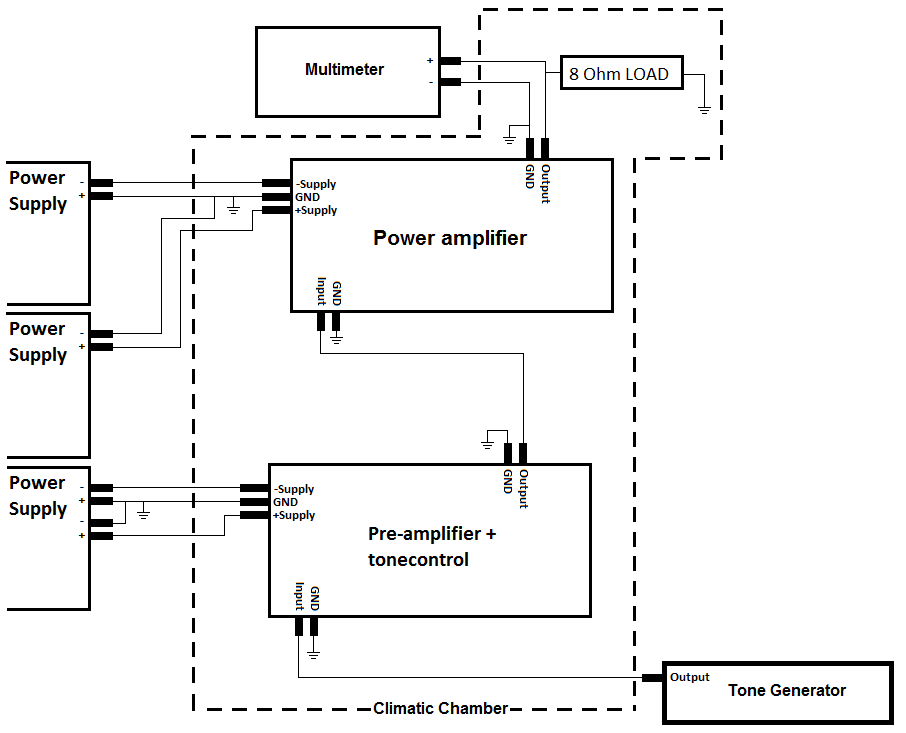
\includegraphics[width=.4\textwidth]{figures/filename}  %<--but is not needed.
  \caption{This image is clearly too small, remember to scale appropriately \fxnote{Remember source}}
  \label{fig:FigureLABEL}  %<--give the figure a label, so you can reference!
\end{figure}               %   For the label to work it must be under the caption.

% Fxnotes will not compile properly inside the figure, only in the caption.
% When \fxnote{} is used in caption, it does not show in a footnote as it normally 
% would, it does however appear in list of corrections.

\autoref{fig:FigureLABEL} $\leftarrow$ use autoref, unless you are referring to multiple pictures, then do like this: \autoref{fig:HbridgeClokwise4Q} and \ref{fig:HbridgeCounterClokwise4Q}.

%Do NOT use \vspace{length}, \hspace{length} or \noindent etc. unless exceedingly necessary - LaTeX is a markup language, let it do its job.
\vspace{.5cm}
\noindent
%
%--------- BIBLIOGRAPHY REF EKSAMPLE -----------------------------------
This reference only represents this line since it is before the punctuation mark\cite{YDing}. This next reference however represents the entire section. That is, all of the preceding sentences in the entire section. This is due to the fact that it is now after the punctuation mark in the end of the section (this is not used in the middle of a section!).\cite{YDing}

%>>PLEASE ALSO READ THE NOTE IN bibliography/bibliography.bib<<

Here is a way to make two images appear on the side of each other. Also, if you modified an image, this is how you properly refer to its original source:

\begin{figure}[H]
    \subcaptionbox  %<--use captionbox instead if no global caption is needed
    {               %                                \%-%-%-%-%-%-%\
      Clockwise 4Q operation.\newline                              %\
      \emph{Edited from image by Biezl.\cite{Biezl}}                %\
      \label{fig:HbridgeClokwise4Q}                                  %\
    }                                                                 %\
    {                                                                  %\
      \includegraphics[width=.46\textwidth]{HbridgeClockwise4Q}         %\
    }                                                                    %\
    \hspace{5pt}                                                          %\
    \subcaptionbox  %<-----------------------------------------------------%\
    {                                                                       %\
      Counterclockwise 4Q operation.\newline                                 %\
      \emph{Edited from image by Biezl.\cite{Biezl}}                          %\
      \label{fig:HbridgeCounterClokwise4Q}                                     %\
    }                                                                           %\
    {                                                                            %\
      \includegraphics[width=.46\textwidth]{HbridgeCounterClockwise4Q}            %|
    }                                                                             %|
    \caption{The 4 quadrant H-bridge configuration shown in both directions.}%<-%-/
    \label{fig:Hbridges}
\end{figure}

As seen \autoref{fig:HbridgeCounterClokwise4Q} can be referred to on its own, or you can use \autoref{fig:Hbridges} to refer to both \autoref{fig:HbridgeClokwise4Q} and \autoref{fig:HbridgeCounterClokwise4Q}.

If the figures are not directly related you might not want to use \textbf{(a)} and \textbf{(b)}, but instead give each figure their own label, here is an example:

\begin{figure}[H]
    \captionbox
    {
      Clockwise 4Q operation.\newline
      \emph{Edited from image by Biezl.\cite{Biezl}}
      \label{fig:HbridgeClokwise4Q2}
    }
    {
      \includegraphics[width=.46\textwidth]{HbridgeClockwise4Q}
    }
    \hspace{5pt}
    \captionbox
    {
      Counterclockwise 4Q operation.\newline
      \emph{Edited from image by Biezl.\cite{Biezl}}
      \label{fig:HbridgeCounterClokwise4Q2}
    }
    {
      \includegraphics[width=.46\textwidth]{HbridgeCounterClockwise4Q}
    }
\end{figure}

In this case \autoref{fig:HbridgeClokwise4Q2} can be referred to without involving \autoref{fig:HbridgeCounterClokwise4Q2}.

\pagebreak			 %|||||||
%			 \section{Table Sample} %to view this sample properly in the code, the screen must be
                       %wide enough, or you have to disable word-wrap in your editor.
\begin{table}[H]
\begin{tabular}{|l|p{5cm}|l|l|l|}
  \hline %-----------------------------------------------------------------------------------
  \textbf{No.} &\textbf{Description} &\textbf{Min} &\textbf{Max} &\textbf{Requirements}    \\
  \hline %-----------------------------------------------------------------------------------
  1            & Some Text           & Some Text   & Some Text   & Some Text               \\
               &                     &             &             & Some More Text          \\
               &                     &             &             & Text Text               \\
               &                     &             &             & Text Text Text          \\
  \hline %-----------------------------------------------------------------------------------
  2            & Some Text           & Some Text   & Some Text   & Some Text               \\
  \hline %-----------------------------------------------------------------------------------
  3            & By specifying the
                 width of a column
                 (|p\{5cm\}|) the
                 cells in that column
                 will not exceed the
                 specified width but         %Extra whitespace is used only for clarity
                 instead expand              %and will not affect the compiled output.
                 downward.
                                     & Some Text           & Some Text   & Some Text       \\
  \hline %-----------------------------------------------------------------------------------
  4            & Some Text           & Some Text   & Some Text   & Some Text               \\
  \hline %-----------------------------------------------------------------------------------
  \multicolumn{2}{|l|}{Some Text}    & \multicolumn{3}{l|}{Some Text}                      \\
  \hline %-----------------------------------------------------------------------------------
  \multicolumn{2}{|l|}{Text Text}    & \multicolumn{3}{l|}{Text = Text}                    \\
  \multicolumn{2}{|l|}{}             & \multicolumn{3}{l|}{Text = Text}                    \\
  \multicolumn{2}{|l|}{}             & \multicolumn{3}{l|}{Text = Text}                    \\
  \multicolumn{2}{|l|}{}             & \multicolumn{3}{l|}{Text = Text}                    \\
  \multicolumn{2}{|l|}{}             & \multicolumn{3}{l|}{Text = Text}                    \\
  \hline %-----------------------------------------------------------------------------------
  \multicolumn{2}{|l|}{Some Text}    & \multicolumn{3}{l|}{Teeeexxtt}                      \\
  \multicolumn{2}{|l|}{}             & \multicolumn{3}{l|}{\LaTeX}                         \\
  \hline %-----------------------------------------------------------------------------------
\end{tabular}
\caption{This Is a Table\label{table:TableLABEL}}
\end{table}

\autoref{table:TableLABEL} $\leftarrow$ use autoref, unless you are referring to multiple tables, then do like this: \autoref{table:TableLABEL} and \ref{table:TableLABEL}.

\pagebreak 		     %|||||||
%			 \section{Equation Sample} %<--In American English all Important Words in
                          %   Headlines are with Big Letters

% \unit is a macro. It uses SI units and aligns all the units neatly :)

\textbf{A normal equation:}
\begin{flalign}
  J_m \cdot \dot{\omega}_m(t) &= \tau_m(t) - B_m \cdot \omega_m(t) - r_m \cdot f_c(t)& \unit{N \cdot m}
  \label{eq:MotorGearNewtonSecLaw}
\end{flalign}
%
\begin{where}
  \va{ J_m               }{is the motor's inertia}                     {kg \cdot m^2}
  \va{ \omega_m(t)       }{is the angular velocity of the motor}       {rad \cdot s^{-1}}
  \va{ \dot{\omega}_m(t) }{is the angular acceleration of the motor}   {rad \cdot s^{-2}}
  \va{ \tau_m(t)         }{is the torque delivered by the motor}       {N \cdot m}
  \va{ B_m               }{is the motor's friction coefficient}        {N \cdot m \cdot s \cdot rad^{-1}}
  \va{ r_m               }{is the radius of the gear, $G_m$}           {m}
  \va{ f_c(t)            }{is the contact force between the two gears} {N}
\end{where}

\textbf{If you need to write something with numbers:} %<--Do not use \textbf{} as headlines, it is bad practice
                                                      %   use instead \chapter{}, \section{}, \subcaption{}, \subsubsection{}
                                                      %   in that order - never a \subsubsection{} directly under a \section{}
\begin{flalign}
  B      &= \num{2,2}\cdot 10^{-6}  \ \si{N\cdot m \cdot rad^{-1} \cdot s}& \label{eq:eq2} \\ %<-- if you want two equations to
  \tau_c &= \num{0.0016}            \ \si{N\cdot m}                       & \label{eq:eq3}    %    allign in one envirenment,
\end{flalign}                                                                              %    remember \\
%using \num{} ensures the same use of decimal point throughout the repport
%should you want to change it, the option is set in the preamble, just change 'period' to 'comma':
%\sisetup{decimalsymbol=period}

\autoref{eq:MotorGearNewtonSecLaw} $\leftarrow$ use autoref, unless you are referring to multiple equations, then do like this: \autoref{eq:eq2} and \ref{eq:eq3}.

\pagebreak		 %|||||||
%			 \section{TikZ Sample}

\textbf{TikZ is only for very patient people, I can recommend Inkscape with textext plugin: \url{https://pav.iki.fi/software/textext/}, difficult to install easy to use, and, if used carefully, nice results.}

%heavily commented example
\input{chapters/tikz/TikZblockDiagramSample.tex}

%way to keep the drawing code in a seperate file
\begin{figure}[H]
	\input{chapters/tikz/smallBlockDiagram.tikz}
	\centering
	\caption{Block diagram}
\end{figure}

%TikZ can also be used for circuits
\input{chapters/tikz/TikZcircuitSample.tex}


\pagebreak            %|||||||
%			 \section{Code Sample}

\begin{lstlisting}[ style=cstyle,
                    caption={C Code}, 
                    label=lst:cExample ]
#include "functions.h"

// Constant matrices
const float L[3] = { -11.0, -12.0, -13.0 };
const float B1[4] = { 0.0, -0.2396, 0.0, 0.2396 };
const float B2[4] = { 0.2396, 0.0, -0.2396, 0.0 };
const float B3[4] = { 0.0377, -0.0377, 0.0377, -0.0377 };
\end{lstlisting}

In \autoref{lst:cExample} is some C-code, and here is some in-line C-code: \inlinec{xTaskCreate();}.

\begin{lstlisting}[ style=pythonstyle,
                    caption={Python Code}, 
                    label=lst:pythonExample ]
# This parses the packets to identify messages and decodes them for the logs
class packetParser():
    def __init__(self,accelfile,gpsfile,measstate,fulllog,plog):
        self.GPS = {0: 'Latitude',
                    1: 'Longtitude',
                    2: 'Velocity'}
        self.IMU = {0: 'AccelerationX',
                    1: 'AccelerationY',
                    2: 'AccelerationZ',
                    3: 'GyroscopeX',
                    4: 'GyroscopeY',
                    5: 'GyroscopeZ',
                    6: 'MagnetometerX',
                    7: 'MagnetometerY',
                    8: 'MagnetometerZ',
                    9: 'Temperature'}
        self.MsgID = {0: self.GPS, 1: self.IMU}
        self.DevID = {0: 'GPS', 1: 'IMU'}
        self.accelburst = [0,0,0,0,0,0,0]
        self.accellog = accelfile
        self.fulllog = fulllog
\end{lstlisting}

In \autoref{lst:pythonExample} is some Python-code, and here is some in-line Python-code:\\ \inlinepython{self.plog.write(str(msgnr))}

\begin{lstlisting}[ style=matlabstyle,
                    caption={Matlab Code}, 
                    label=lst:matlabExample ]
  close all
  clear
  clc
  
  % Parameters
  mx=200;     % [kg] mass + added mass in xb direction
  my=250;     % [kg] mass + added mass in yb direction
  Iz=700;     % [kgm2]
  
  dx=70;      % [kg/s] 
  dy=100;     % [kg/s]
  dyaw=50;    % [kgm2/s]
\end{lstlisting}

In \autoref{lst:cExample}, \ref{lst:pythonExample} and \ref{lst:matlabExample} is some code, and here is some in-line matlab: \inlinematlab{randn(50)}            %|||||||
%|||||||                                                 ||||||||
%||||||||||||||||||||||||||||||||||||||||||||||||||||||||||||||||
%||||||||||||||||||||||||||||||||||||||||||||||||||||||||||||||||


%%% Prereport %%%
		\setlength\cftaftertoctitleskip{2pt}
		\setlength\cftafterloftitleskip{6pt}
		\setlength\cftafterlottitleskip{6pt}
%\selectlanguage{danish}
%\title{Testing the performance of linear regressors using inertial information combined with sEMG to minimize the limb position effect in proportional and simultaneous control of lower arm prosthetics.}

%%% Frontmatter Settings %%%
		\pagestyle{empty} %disable headers and footers
		\pagenumbering{roman} %use roman page numbering in the frontmatter I II...
%		\fancyfoot[RE,LO]{17gr7404} %page number on all pages
%		\fancyfoot[LE,RO]{\thepage}
%		\fancyhead[LE,LO,RE,RO]{}

%%% Introductory Formalities %%%
%\includepdf[pages={1}]{formalities/frontpage.pdf}
%			\clearpage
\thispagestyle{empty}

\begin{figure}[H]
	\raggedleft
	
\includegraphics[width=0.2\textwidth]{figures/aaulogo-en.png}
\end{figure} 

\vspace{5 cm}

\begin{center}
	\begin{Huge}
		\textbf{Examining if Confidence Score Feedback During User Training Can Improve Users’ Ability in Controlling Upper Limb Prosthetics}\\
		\vspace{5 mm}
		2nd semester Masters, Biomedical Engineering \& Infomatics - Spring $2018$\\
		\vspace{3 mm}
	\end{Huge}
	{\Large Project group: $18$gr$8408$} \\
	\vspace{1cm}
	\large{Simon Bruun, Oliver Thomsen Damsgaard, Martin Alexander Garenfeld, Christian Korfitz Mortensen}
\end{center}
\vspace*{\fill}

\begin{center}
	\line(1,0){400}
\end{center}

%\newpage
%
%\large{\textbf{Project period:}\\
%P7, Autumn 2017\\
%01/08/2017 - 20/12/2017\\
%
%\textbf{Project group:}\\
%17gr7404\\} %\fxnote{Input group number}
%
%
%\begin{center}
%	\Large{\textbf{Collaborators:}\\
%		\vspace{1.5cm}
%	\rule{10cm}{1pt}\\
%	Irene Uriarte \\
%	
%	\rule{10cm}{1pt}\\
%	Martin Alexander Garenfeld \\
%	
%	\rule{10cm}{1pt}\\
%	Oliver Thomsen Damsgaard \\
%	
%	\rule{10cm}{1pt}\\
%	Simon Bruun \\}
%\end{center}
%
%
%
%\large{\textbf{Supervisors:}\\
%Strahinja Dosen \\
%Jakob Lund Dideriksen \\
%Lotte N.S. Andreasen Struijk} \\
%\\
\newpage
			% <--- the frontpage
%			\pagestyle{fancy}
%%{\small
\strut\vfill % push the content to the bottom of the page
\noindent Copyright \copyright{} Aalborg University 2015\par
\vspace{0.2cm}

\noindent This report is compiled in \LaTeX, originally developed by Leslie Lamport, based on Donald Knuth's \TeX. The main text is written in \emph{Latin Modern} pt 12, designed by Bogusław Jackowski and Janusz M. Nowacki. 
%The document is compiled via the website \url{www.overleaf.com}, an online collaborative based \LaTeX-editor with instant preview, which enables multiple persons to edit the document simultaneously.
Flowcharts and diagrams are made using Microsoft Visio. 
\clearpage
%			%\begin{document} 
\thispagestyle{empty}
\begin{titlepage}
\begin{nopagebreak}
{\samepage 

\begin{tabular}{r}
\parbox{\textwidth}{  \raisebox{-15mm}{
\includegraphics[height=3cm]{figures/aaulogo-en.png}}
\hfill \hspace{2cm} \parbox{8cm}{\begin{tabular}{l} %4.90
{\small \textbf{\textcolor{aaublue}{{7\textsuperscript{th} Semester, Masters Project}}}}\\
{\small \textbf{\textcolor{aaublue}{School of Medicine and Health}}}\\
%{\small \textbf{\textcolor{aaublue}{Communication Technologies}}}\\ 
{\small \textbf{\textcolor{aaublue}{Biomedical Engineering and Informatics}}}\\
{\small \textcolor{aaublue}{Fredrik Bajers Vej 7A}} \\
{\small \textcolor{aaublue}{9220 Aalborg}} \\
%{\small \textcolor{aaublue}{\emph{http://www.sict.aau.dk/electronics-and-it}}}
\end{tabular}}}
\end{tabular}

\begin{tabular}{cc}
\parbox{7cm}{

\textbf{The effect of limb position on myoelectric prosthetic control using linear regression}
\\
\textbf{Theme: Biomedical signals and information}

\small{
\\
}


\parbox{8cm}{


\textbf{Project period:}\\
P7, Autumn 2017\\
01/08/2017 - 20/12/2017\\
   
\textbf{Project group:}\\
17gr7404\\ %\fxnote{Input group number}
  
\textbf{Collaborators:}\\
\rule{5cm}{1pt}\\
Irene Uriarte \\
\rule{5cm}{1pt}\\
Martin Alexander Garenfeld \\
\rule{5cm}{1pt}\\
Oliver Thomsen Damsgaard \\
\rule{5cm}{1pt}\\
Simon Bruun \\

\textbf{Supervisors:}\\
Strahinja Dosen \\
Jakob Lund Dideriksen \\
Lotte N.S. Andreasen Struijk \\
}\\


\textbf{Pages:} 0\\
\textbf{Appendixes:} b \\
%\textbf{Ekstra:} For projektkode: Se forord\\ %eks. en CD eller USB
\textbf{Completed:} 19/12/2017\\

\vfill } &
\parbox{7cm}{
  \vspace{.15cm}
  \hfill
  \begin{tabular}{l}
  {\textbf{Abstract}}\bigskip \\
  \fbox{
    \parbox{6.5cm}{\bigskip
     {\vfill{\small \lipsum[15]
%write real thing
     \bigskip}}
     }}
   \end{tabular}}
\end{tabular}} %\vspace{1cm}


\centering
\textit{Publication of this report's contents, including source references, may only happen in agreement with the authors.}\\
%\textit{Offentliggørelse af rapportens indhold, med kildeangivelse, må kun ske efter aftale med forfatterne.}\\


\end{nopagebreak}
\end{titlepage}
%\end{document} 			 % <--- the titlesheet - contains the synopsis!!
%%%% Preface %%%
%			\cleardoublepage
%			%abstract

%\section{Abstract}					%prolly not needed

%clever abstract below
The user rejection rate of myoelectric prosthetics is currently high, due to slow and inaccurate control. Previous studies have shown user training to be an important part of overcoming the challenge of making transradial upper limb prosthetics more accurate, as the control systems depend on the user generating the same distinguishable muscle patterns when using the prosthesis. Different methods have been sought when adapting users to perform specific distinguishable movements. This study aimed to investigate whether confidence score feedback from a LDA classifier during user training could improve user performance in a Fitts' Law test compared to a control group who only received label feedback. %The study will be designed to examine prosthetic control in lower arm prosthetics.
16 able-bodied subjects were recruited for the study; 8 subjects randomly assigned to each group. Each subject went through a three session experiment; one session per day over three consecutive days. During each session the subject received a 16 minutes user training and went subsequently through a Fitts' Law test to evaluate the performance.
%, where they were instructed to perform six different hand movements in three intensities during data acquisition. This was then used to build a LDA based classifier the subjects were to use during the training, teaching them to perform specific movements at different intensities. Afterwards they were subjected to a Fitts' Law based test in a GUI to examine their ability to perform the trained movements. These steps were repeated for three sessions over three consecutive days.
A significant improvement in cluster dispersion of EMG signals of separate movement was found in the control group, where the third session resulted in more dense clusters both when compared to the first session of the control group and third session of the test group. The results from the Fitts' Law test showed no significant difference between the two groups and no improvement over the three sessions for either of the groups. Overall, three sessions of user training with confidence score feedback showed to be an insufficient training period to observe a significant improvement within and between subject groups.

\textit{\textbf{Keywords: surface electromyography, lower arm prosthetics, linear discriminant analysis, user training, confidence scores}}			 % <--- this is the abstract!!
%%\clearpage
%			\chapter*{Preface}

\lipsum[9]

\pagebreak				% <--- the preface
%
%			\pdfbookmark[0]{Table of Contents}{label: tableOfCentents}
%			\tableofcontents
%%			\cleardoublepage


%%% Mainmatter Settings %%%
\pagenumbering{arabic} %use arabic page numbering in the mainmatter
\fancyhf{}
\fancyfoot[C]{\thepage} %\text{ of} \pageref{LastPage}}
%\fancyfoot[RE,LO]{17gr7404}
%\fancyhead[RE,LO]{}
%\fancyhead[RE,LO]{\color{aaublue}\small\nouppercase\leftmark} %even page - chapter title
\pagestyle{fancy}


%---------------------------INPUTS-------------------------------

%%statusseminar text

\chapter*{Using estimation uncertainty to improve prosthesis control}

\textbf{Group 8408. Simon Bruun, Oliver Damsgaard, Martin Garenfeld, Christian Mortensen}

\section*{Introduction}

Electromyography (EMG) is the recording and utilization of muscle generated electric potentials, widely used in control of functional prosthetics. The electric potentials recorded from the muscles are action potentials generated by the activation of a muscle contraction. The contraction force a muscle produce is related to the intensity of an EMG recording. The recorded EMG signals are processed through several steps of amplification, filtering and feature extraction before they are used as input in the control for a myoelectric prosthesis. \cite{Cram2012, Fougner2012}

Myoelectric prosthetics are becoming increasingly advanced, however they still suffer commercial success due to lack of usability outside clinical environments. \cite{Hwang2017, Jiang2012, Scheme2010} Thus, many users reject the use of the prosthetics. 
In recent years development in myoelectric prosthetics have been greatly focused on refining classification accuracy, while other research areas have been more or less neglected \cite{Jiang2012}. However, there still exist a challenge for the users to be able to consistently produce distinguishable muscle patterns, and the better these muscle patterns the better the system will function. \cite{Powell2014} Far fewer studies have been made on user training when compared to studies on system training, though the significance of user training is not doubted \cite{Fang2017}. Powell et. al conclude that in order for amputees to understand the significance of producing consistent and distinguishable muscle patterns, the need for user training is important \cite{Powell2013}.

Fang et. al \cite{Fang2017} evaluated the progress of the human learning ability in a pattern recognition based control scheme when providing classifier-feedback during user training. Here, a clustering-feedback method based on Principal Component Analysis (PCA) was used to provide users with real-time visual feedback, to guide users to correctly perform movements based on the recorded EMG signals. The visual feedback consisted of a map with dots representing centroids of classes. Through control based on an Linear Discriminant Analysis (LDA) classifier, users could match the control input to these centroids to best perform a movement to be classified correctly. The study showed great improvements for user training, and an ability to quicken the learning for amputees who are unfamiliar with EMG controlled prosthetic use. \cite{Fang2017}
Powell et. al \cite{Powell2014} demonstrated, by using an LDA classifier, an increase in movement completion percentage from 70.8\% to 99.0\%, a decrease in movement completion time from 1.47 to 1.13, as well as a significant improvement in classifier accuracy from 77.5\% to 94.4\%, for users undergoing user training for a two week period. This study provided feedback through a virtual animated prosthesis.
Pan et. al \cite{Pan2017} provided a visual feedback of an arrow to be moved on a 2D plane. Pan et. al also tested the effect of stimulating the subjects’ brain with transcranial direct current stimulation (tDCS). The study concluded that tDCS together with user training provided significantly better results than user training alone. \cite{Pan2017}

The general challenge of user training is for the user to be able to consistently produce distinguishable muscle patterns. \cite{Powell2014} Therefore further research in user training could provide a vital leap towards more precise classification using current methods, as well as a faster user adaptation of myoelectric controlled prosthetics, but an effective way to properly provide feedback to the user have yet to be developed. 
Further studies should for now concentrate on developing different feedback methods which should later be compared to determine an ideal method. 
This study will seek to develop a new method of feedback during user training, by providing the users with the estimation uncertainty of the classification. To the authors knowledge, user feedback has not been provided with this method before.

\section*{Methods}

%This study will utilize classification and probability estimation based on EMG recordings to evaluate and compute uncertainty estimations for classifying four different hand gestures. The goal is to develop a system that use the classification uncertainties to improve user training.

%The study will consist of steps of data acquisition, user training and an online test. The user will undergo user training followed by a targets reaching Fitts' Law test. The study will have a test and control group, where the control group will be trained without visual feedback during user training. Post hoc statistic comparisons will be made between online tests and maybe some other things we have not entirely decided upon yet.

\textbf{Data acquisition} will be done with a Myo armband (MYB) from Thalmic Labs. The MYB contains eight surface EMG electrodes, which has a sampling rate of 200 Hz.
For \textbf{feature extraction} four features will be extracted from the acquired data; slope-sign changes (SSC), waveform length (WL), zero crossings (ZC) and mean absolute value (MAV). The features will be extracted from a window of 200 ms (40 samples) with a 50\% overlap.
For \textbf{classification} LDA will be used. LDA is a supervised classification method used to separate classes of data by linear decision boundaries. Classification methods attempt to classify similar patterns in EMG signals, between previously acquired data and new data \cite{Mendez2017}. In LDA each decision boundary is a hyperplane from which the minimum distance from the classes it separates is maximized, and the distance from the means of the classes are maximized. A decision boundary is defined as a linear combination of the feature values.
Evaluating the certainty that a feature value belongs to a given class can be done by computing the posterior probability of each class. The posterior probability is a value between 0 and 1. The posterior probability is given as the product of the class conditional probability and the prior probability divided by a normalization term that guaranties that the posterior probabilities for all classes sums to one. The class conditional probability is the probability of obtaining a feature value when selecting samples randomly from a class. The prior probability is the likelihood that a sample from a class appears when compared to the other classes before it actually has appeared.

The effect of user training with and without providing uncertainty estimations during the user training, will be tested through a target reaching test. The test will executed in a virtual environment. During the test the user must reach targets of varying size and distance to each other. The test evaluates users speed to reach targets, accuracy, overshoot and overall completion rate \cite{Scheme2013}. 
Lastly a \textbf{statistical} analysis will be used to compare results of the target reaching test between users training with and without provided estimated uncertainty during user training.


\section*{Study protocol}

\textbf{Research question/hypothesis}

Using uncertainty estimation as visual feedback during user training will improve the users performance in a linear discriminant controlled target reaching test based on electromyography recordings.

\textbf{Ethical considerations}  

The investigators do not foresee any obstacles of ethical nature during the proceedings of this experiment. No test subjects will be exposed to any physical interventions besides being asked to wear the Myo armband. No part of this experiment should put the subject in danger. 

\textbf{Session time}

The experiment consist of one session divided into two sub-sessions with an estimated total duration of 2-3 hours.

\textbf{Inclusion criteria}

The subject needs to be:
\begin{itemize}
	\item able bodied.
	\item between 18 and 35 years of age.
	\item able to understand and speak Danish and/or English.
	\item assessed by the investigators to understand and perform the instructions given during the experiment. 
\end{itemize}


\textbf{Exclusion criteria}

The subject must not have:
\begin{itemize}
	\item diseases that, assessed by the investigators, might influence subject performance.
\end{itemize}


\textbf{Experiment procedure}

The experiment is divided into two sessions: 1) training data acquisition, user training and performance test and 2) new training data acquisition and performance test. During the training data acquisition EMG data will be recorded from the subject with an EMG-electrode armband (Myoband from Thalmic Labs) when performing four different wrist movements (flexion, extension, radial deviation and ulnar deviation). The data is subsequently used to fit a classification model used in the myoelectric control scheme for the following user training and performance test. Before the performance test the user is given a training period to get familiar with wrist movements used in the performance test. During the performance test the subject will perform a target-reaching task in a cartesian coordinate system of reaching a number of targets using wrist movements, where each axis represent a one of four wrist movements. The aim for the subject is to reach as many targets as quickly as possible. The subject will perform the target-reaching task twice - one in each session. The subjects are divided into two groups: a test group and a control group. As the study is single-blinded the subject will not be informed which group he/she belongs to.

\begin{figure}[H]                                         
	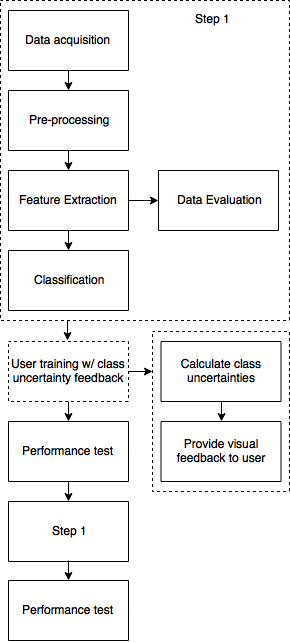
\includegraphics[width=.4\textwidth]{figures/sStatusSeminar/systemPepeLineTG}  
	\caption{System pipeline for the test group. The following chronology describes the steps in greater detail.}
	\label{fig:sysPipeTG} 
\end{figure} 


Chronology of session 1, for subjects in the test group:
\begin{enumerate}
	\item Apply Myoband on dominant forearm at the thickest part.
	\item Synchronize Myoband by performing wrist extension until three distinct vibrations are felt.
	\item Perform 15 seconds of maximum voluntary contraction (MVC) of instructed movement. Following the MVC the subject will be given a 30 resting period to avoid fatigue.
	\item Perform 15 seconds contractions of respectively 40\%, 60\% and 70\% of MVC. During these contractions the subject will control a green marker representing the EMG signal and try to follow a trapezoidal trajectory a precise as possible. The trapezoidal trajectory consists of two five second transition phases and one five second plateau phase. Between each trial the subject will be given a 15 seconds resting period to avoid muscle fatigue.
	\item Repeat step 3-4 until training data from all four wrist movements has been recorded.
	\item The subject will train the four wrist movements. Each movement will be performed 10 times, where each single movement consists of a five second movement with increased intensity. To improve the precision of movements the subject will receive visual feedback consisting of the probability the movement to belong to based on the classifier. The ideal probability during the training is a 100\% probability of belonging to the trained movement and a 0\% probability of belonging to the remaining movements. 
	\item The subject will perform a target-reaching test. The subject will control a cursor in a cartesian coordinate system representing the output of the LDA classifier. To complete a target the subject must dwell the cursor within the target for 0.5 seconds. If this is achieved the target will disappear. The target will similarly disappear if the subject fails to achieve this within 15 seconds. When a target disappears a new target appears for the user to reach. This procedure is continued until no more targets are shown. After finishing the performance test the subject will be given a 2 minutes resting period.
\end{enumerate}


Chronology of session 2, for subjects in the test group:
\begin{enumerate}
	\item Perform step 3-5 from session 1.
	\item Perform step 7 from session 1. 
\end{enumerate}

The sessions for subjects in the control group will follow that of the test group with the exclusion of the provided estimation uncertainties during step 6.

\clearpage








\chapter{Introduction}

%paper introduction

\section{Introduction}			%skal måske fjernes afhængigt af hvordan vi sætter main op

%    https://www.youtube.com/watch?v=BzVmPsqHDDQ
Electromyography (EMG) is the recording of muscle generated electric potentials, widely used in control of functional prosthetics. The electric potentials recorded from the muscles are action potentials generated before the inception of a muscle contraction. The contraction force a muscle produce is related to the intensity of an EMG recording. The recorded EMG signals are processed through steps of amplification, filtering and feature extraction before they are used as input in the control for a myoelectric prosthesis. \cite{Cram2012, Fougner2012} %For the actual control of the prosthetics several different methods for control schemes exist.

%the best introduction including the great works of Jiang \cite{Jiang2012} to say that an overall problem with myoelectric prosthetics exist in the fact that not everything has yet been investigated. However this should be done in order to know everything. Everything should be researched. 

Ever increasingly advanced myoelectric prosthetics and control systems are being developed. Despite the efforts a critical bottleneck still exist: the ability to properly control the advanced prosthetic \cite{Hwang2017}. In relation to pattern recognition methods the overall challenge lies in the ability for the system to be able to recognizing the muscle patterns produced by the user. Control systems have become exceedingly good at correctly estimating muscle patterns. However, there still exist a challenge for the users to be able to consistently produce distinguishable muscle patterns, and the better these muscle patterns the better the system will function. \cite{Powell2014}

In recent years the research area of myoelectric prosthetics has been dominated by classification methods for control schemes. Classification attempts to classify similar patterns in EMG signals, between previously acquired data and new data \cite{Mendez2017}. Classification enables proportional control of trained movements in several degrees of freedom (DOF), but but only a single movement a time. The classification control scheme has lacked usability outside of clinical environments \cite{Scheme2010}, which has resulted in scarce commercial success \cite{Jiang2012}.
%Recently regression methods have been gaining more interest as a control scheme for myoelectric prosthetics. Regression methods provide a continuous output value, contrary to classification which provides a single class per movement \cite{Hahne2014}. Regression methods have shown promising results of robust control while performing both proportional and simultaneous movements \cite{Hwang2017, Hahne2014}. This shows potential for regression based control schemes to be more reliable when used for performing daily life tasks outside clinical environments.However, the regression-based control approach lacks accurate control when performing delicate movements or when the user only desires to perform a single movement in one DOF. [cite til 7.semester projekt].

Many advancements have been made on system training to improve the systems and control schemes to best recognize the performed movements by the users. Jiang et. al \cite{Jiang2012} determine that a change of focus in the myoelectric prosthetics research area should be made. Perhaps as a result of a too single-minded approach in the research community, compared to system training, far fewer studies have investigated the effect of user training. 
Improving the users ability to properly utilize the system is the goal of user training. Here, an important consideration is that each user will have individual competences when initiating user training. Some might perform well from the beginning while others will show little to no success. \cite{Powell2013} Powell et. al \cite{Powell2013} conclude that in order for amputees to understand the significance of producing consistent and distinguishable muscle patterns, the need for user training is important. User training can help amputees to gain the skill of controlling pattern recognition based prosthetics and to later adopt the use of one such prosthesis \cite{Powell2013}.

The significance of user training is not doubted, and several different approaches has been investigated. Fang et. al \cite{Fang2017} evaluated the progress of the human learning ability in a pattern recognition based control scheme when providing classifier-feedback during user training. Here, a clustering-feedback method based on Principal Component Analysis (PCA) was used to provide users with real-time visual feedback, to guide users to correctly perform movements based on the recorded EMG signals. The visual feedback consisted of a map with dots representing centroids of classes. Through control based on an Linear Discriminant Analysis (LDA) classifier, users could match the control input to these centroids to best perform a movement to be classified correctly. The study showed great improvements in performance after user training, and an ability to quicken the learning for amputees who are unfamiliar with EMG controlled prosthetic use. \cite{Fang2017}
Other studies have also showed promising results using an LDA classifier during user training. Powell et. al \cite{Powell2014} demonstrated an increase in movement completion percentage from 70.8\% to 99.0\%, a decrease in movement completion time from 1.47 to 1.13, as well as a significant improvement in classifier accuracy from 77.5\% to 94.4\%, for users undergoing user training for a two week period. This study provided feedback through a virtual animated prosthesis.
Pen et. al \cite{Pen2017} provided a visual feedback of an arrow to be moved on a 2D plane. Pen et. al also tested the effect of stimulating the subjects brain with transcranial direct current stimulation (tDCS). The study concluded that tDCS together with user training provided significantly better results than user training alone. \cite{Pen2017}

The general challenge of user training is for the user to be able to consistently produce distinguishable muscle patterns. \cite{Powell2014} Therefore further research in user training could provide a vital leap towards more precise classification using current methods, as well as a faster user adaptation of myoelectric controlled prosthetics, but an effective way to properly provide feedback to the user have yet to be developed. 
%Further studies should for now concentrate on developing different feedback methods which should later be compared to determine an ideal method. 
This study will seek to develop a new method of feedback during user training, by providing the users with the confidence scores of a LDA classifier as used in \cite{Scheme2013} for a confidence-based rejection system control scheme, and the level of contraction of the performed movement as proposed in \cite{Englehart2003}. To the authors knowledge, these feedback parameters have not yet been provided in a combination in user training for myoelectric prosthesis users. %Initially the study will propose providing feedback via a bar chart each bar representing the estimated uncertainty of a classified movement. 

%The following section ought to be a overview section in the beginning of the method section:
%The study will consist of steps of data acquisition, user training and an online test. The user will undergo user training followed by a targets reaching Fitts' Law test. The study will have a test and control group, where the control group will be trained without visual feedback during user training. Ad hoc statistic comparisons will be made between online tests and maybe some other things we have not entirely decided upon yet. /cite(we decide)

The remainder of this paper will be structured in "x numbers" of sections. Section 2 will further describe the experimental setup, subject management and experimental protocol. Section 3 will describe the methods used to do something with the control off and the user training thing we do. Section 4 present the result, discussion and conclusion. 



\chapter{Background}

%anatomy
\section{Choice of Movements} \label{sec:BG:anatomy}
%\section{Anatomy of the distal part of the arm} \label{sec:anatomy} 		%%old

%arguments for choice of movements (header)
%anatomy/physiology of arm and muscles
%segue to EMG

%head
This project will use six movements based on three degrees of freedom (DOF) for control of a virtual interface. The movements are extension, flexion, radial and ulnar deviation, closed and opened hand as well as rest. The movements are shown in \figref{fig:handMovements}. %These six movements cover DOFs which will be used in the control scheme for testing performance in a virtual target reaching test, described in \secref{sec:fitts}. 
These movements are distinguishable from each other and therefore very useful in classification. % either individually or in combination most often used during many daily life tasks. Thus 
Training users to improve performance of these movements for use in a myoelectric prosthesis control scheme, could give a good foundation to build a classification scheme upon. %Other movements such as supination and pronation of the the hand have been considered, but the seven chosen movements performed by muscles active in the upper muscle layer of the forearm, and would thus
%enable a good classification  prove to cover most functions a prosthesis should cover for use in daily life tasks. 

%In this project recordings of EMG signals will be used for control and test of the effect of providing class certainty feedback during user training. The recordings will be made with a Myo armband (MYB) described in \secref{sec:MYB}. The recordings will be recorded from the lower forearm of test rejects on muscles involved with performing the six different stated movements. 

\begin{figure}[H] 
	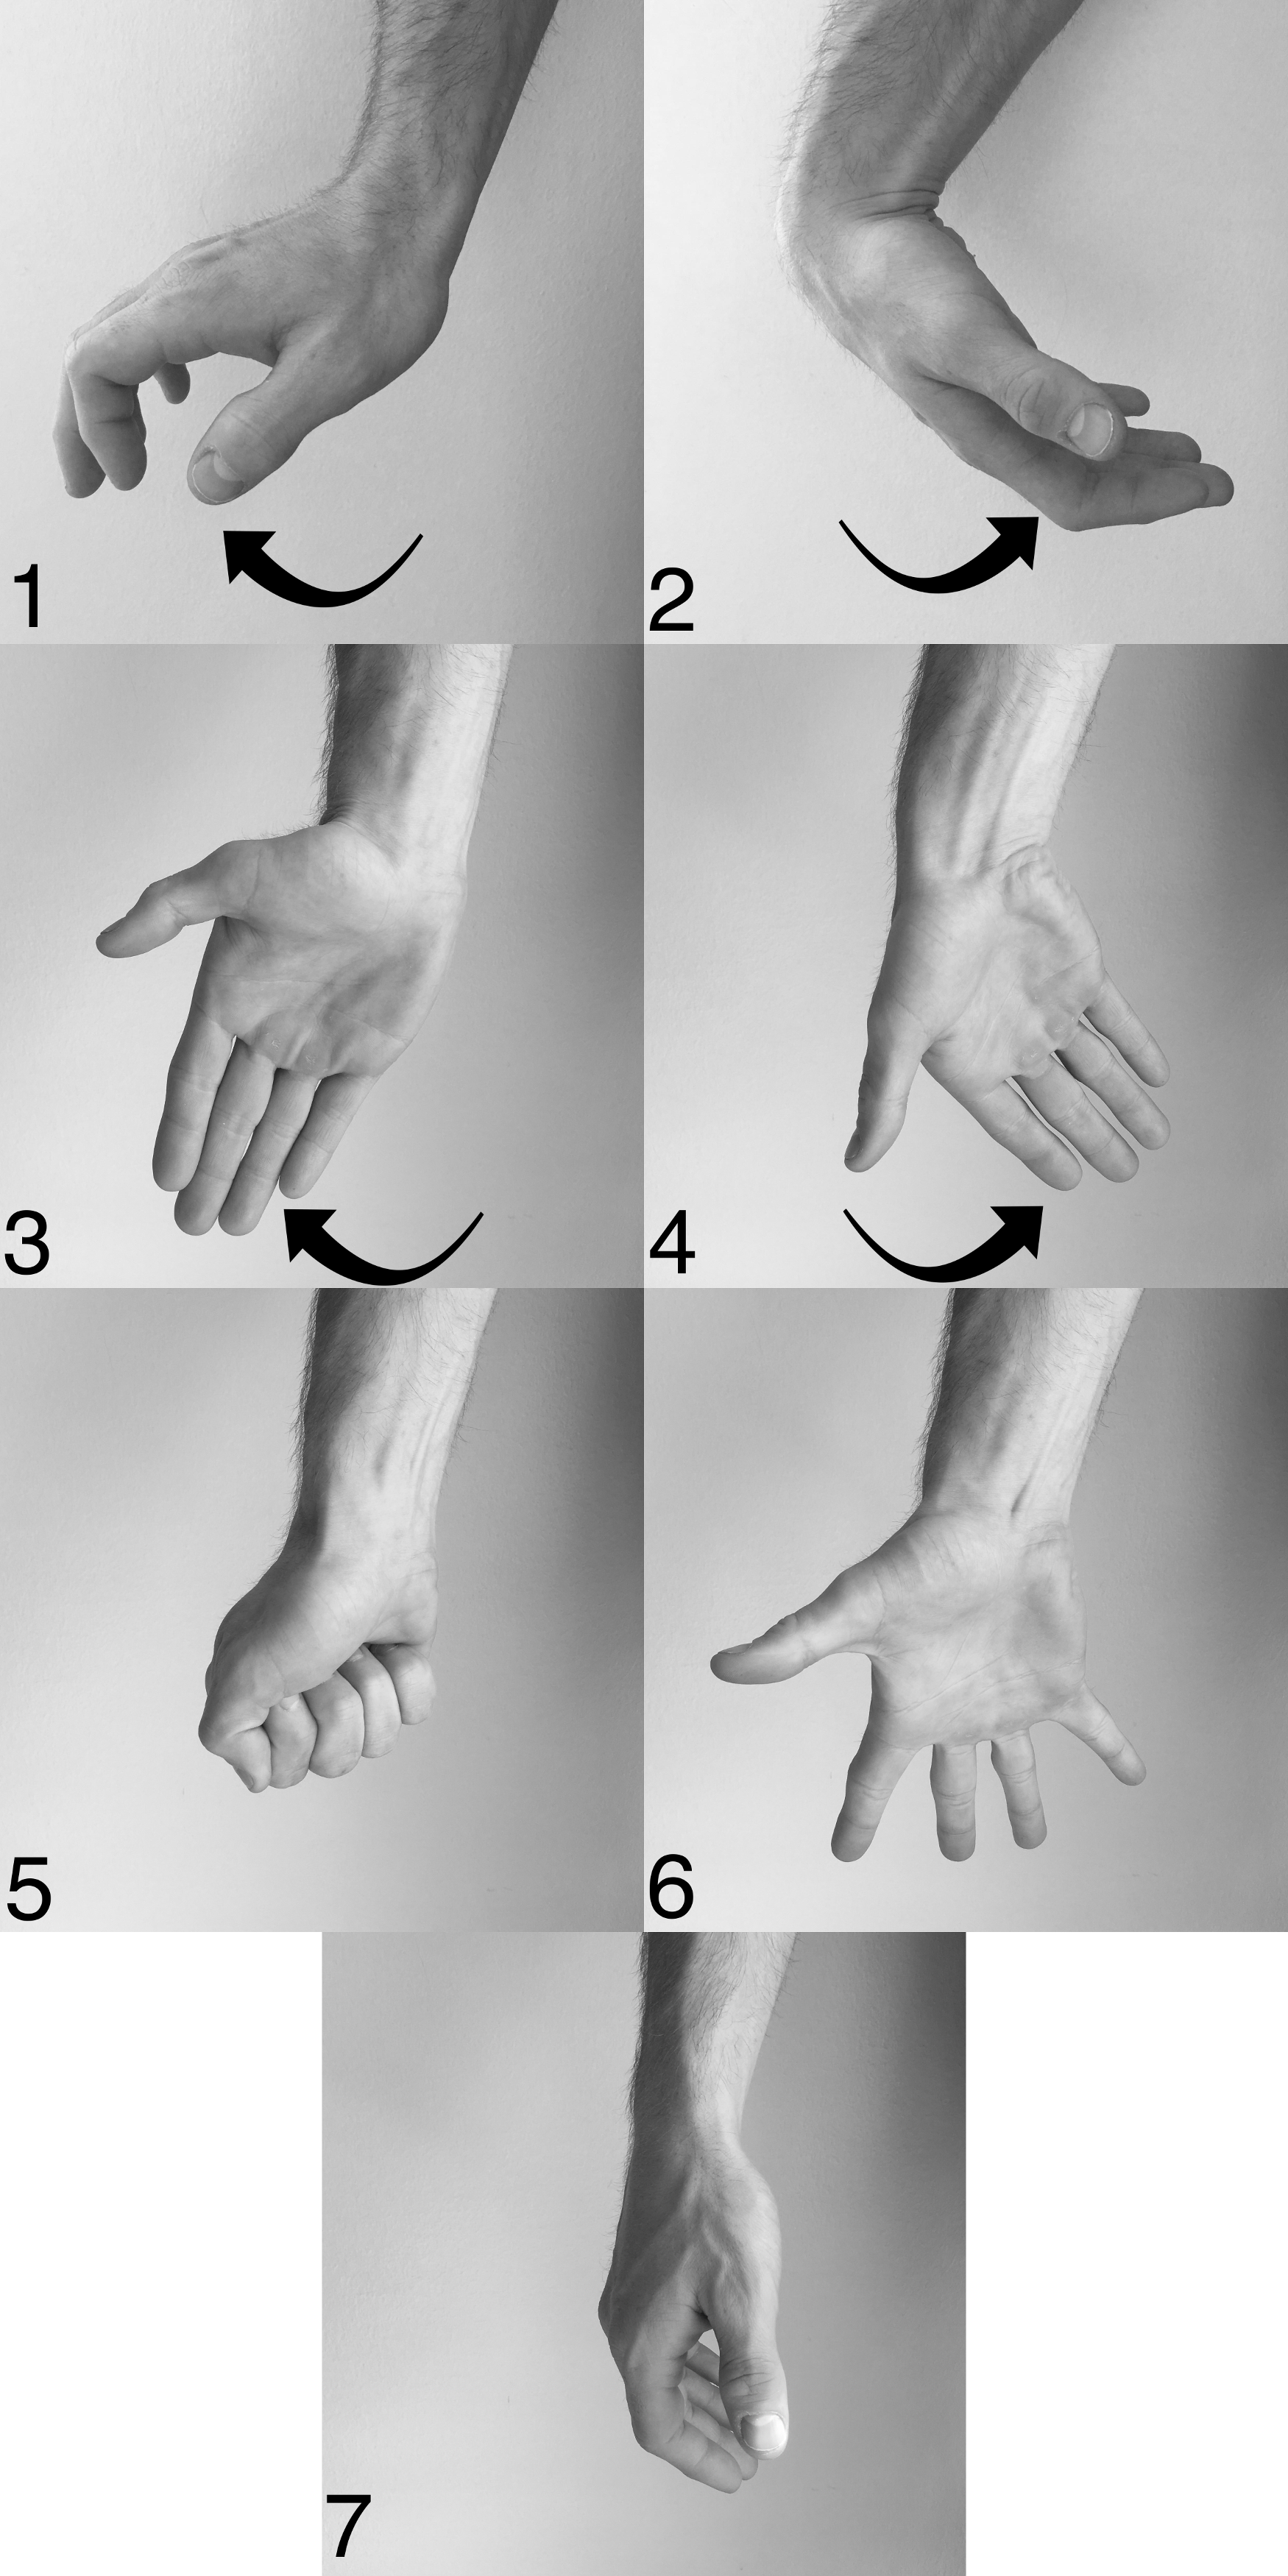
\includegraphics[width=0.4\textwidth]{figures/handGestures/BW/allHandMovementsVerticalBW}
	\caption{The figure shows the six hand movements used in this study as well as rest. The movements are: 1) extension, 2) flexion, 3) radial deviation, 4) ulnar deviation, 5) closed hand, 6) opened hand and 7) rest.}
	\label{fig:handMovements}
\end{figure}

%The human arm has five DOFs being covered by the movements extension, flexion, abduction, adduction and rotation at the shoulder, flexion at the elbow and supination and pronation of the lower forearm. 
%Three of the five DOFs covered by movements at the shoulder is illustrated in \figref{fig:armMovements}.

%\begin{figure}[H] 
%	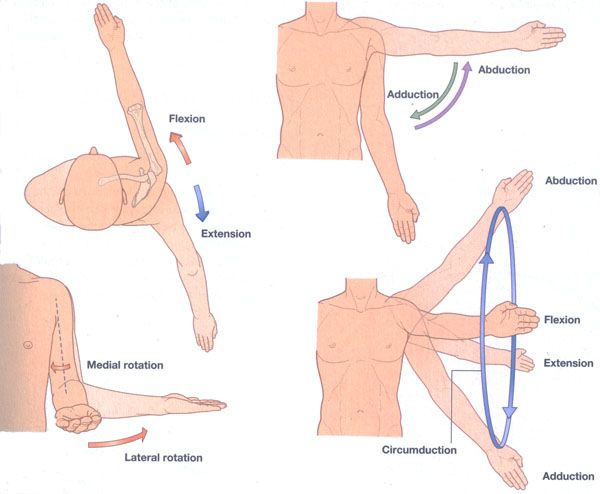
\includegraphics[width=0.5\textwidth]{figures/xBackground/aAnatomy/armMovements}
%	\caption{Movements at the shoulder: extension, flexion, abduction, adduction and rotation in medial and lateral direction. The movements cover three of the five DOFs of the arm. \cite{Kim2015}}
%	\label{fig:armMovements}
%\end{figure}

%The human hand is a very versatile and dexterous apparatus possessing a total of 25 active DOFs. These DOFs are expressed at the fingers, wrist and palm, where the fingers account for a total of 21 DOFs and the wrist account for two DOFs. Each finger posses four DOFs, while the thumb has five, also being able to do opposition movement to each other finger. At the wrist the hand can flex and extend as well as perform radial and ulnar deviations. The last two DOFs exist in the palm of the hand where the joints between the fourth and fifth metacarpal bones and the hamate bone of the carpal bones in the wrist give the hand movement along two additional axes which is used when doing opposition of the thumb and the fifth finger. \cite{Martini2012}

%Many of these DOFs and corresponding movements are active when using the hand. The chosen movements for this project will involve most of the DOFs in the hand, as can be seen on \figref{fig:handMovements}. Movements at the wrist (extension/flexion, radial/ulnar deviation) are DOFs of the hand. Even though many individual movements of joints and DOFs of the hand and fingers are active during opening and closing of the hand. During the rest of the project these two movements will be described as being movement in one DOF. 

%\subsection{Muscles of the lower forearm} \label{sec:BG:musclesOfTheArm}

To perform movements of the wrist anf fingers, many muscles in the forearm are activated. All movements relevant for this study are controlled by muscles in the forearm, as well as some in the palm of the hand. However, as EMG recordings will be done from the forearm by equipment described in \secref{sub:BG:MYB}, it is relevant to gain knowledge on the muscles in the forearm. 
When performing actions at the wrist the following muscles are active: flexor carpi radialis, flexor carpi ulnaris, palmaris longus, extensor carpi radialis longus, extensor carpi radialis brevis, extensor carpi ulnaris. The flexor and extensor muscles are naturally responsible for performing flexion and extension respectively at the wrist. They are however also responsible for performing radial and ulnar deviation, where the flexor carpi radialis and extensor carpi radialis brevis muscles, which are antoganistic muscles when doing flexion and extension, will work together when performing radial deviation. The extensor carpi radialis longus muscle is also responsible for performing radial deviation. The flexor and extensor carpi ulnaris muscles are responsible when performing ulnar deviation. The palmaris longus muscle is only active during flexion at the wrist. \cite{Martini2012}

Several more muscles are further specified to perform movements of the fingers but many of these are also active during extension/flexion and radial/ulnar deviations at the wrist. Muscles responsible when opening the hand by extending the fingers are: extensor digitorum, extensor pollicis brevis, extensor pollicis longus, extensor indicis and the extensor digiti minimi muscle. Contrary, the muscles responsible for closing the hand by flexing the fingers are: flexor digitorum superficialis, flexor digitorum profundus and the flextor pollicis longus. \cite{Martini2012}







%being able to perform extension, flexion at both its joint between the distal/proximal phalanges and proximal phlanges and metacarpal bone. It can perform abducation, adducation, fl
%
%
%%EMG recordings will be measured from the distal forearm of test subjects, in order to use EMG signals for control and test the effect of providing feedback during user training. Recordings will be recorded with a Myo armband (MYB) from Thalmic Labs, further described in \secref{sec:MYB}. This section will provide information on the anatomy of the distal part of the arm and the general muscles involved in movements used in this project.\\
%
%
%The human arm is the base and extender for our greatest tool: the hand. The human hand is a very versatile and dexterous tool, and the loss of that function is therefore a great loss in relation to functionality and independence. The hand gains its vast utilization by having 27 degrees of freedom (DOF). This in itself makes it very dexterous but it is the arm that moves the hand along seven DOFs, that enables the hand to use its dexterity.\\
%Movement of limbs are caused by muscle contractions. The muscles contract when receiving nerve impulses from the central nervous system (CNS). \cite{Martini2012} \\
%The greater workings of muscle activation is described further in \secref{sec:EMG}.  
%Many muscles in the lower forearm are involved when performing hand gestures. Several muscles are actors in performing specific movements, and some of these are at times antagonistic muscles but will work together when performing other movements. The flexor carpi radialis and extensor carpi radialis brevis muscles are as an example antagonists in performing flexion and extension at the wrist, but are both involved when doing abduction of the wrist. \cite{Martini2012} 
%NO -- This can prove a problem when recording EMG signals from these muscles, since if based only on the recording there is no way of knowing which muscle and under which movement the signal is recorded from. However, this problem is overcome when doing EMG recordings of several muscles at the same time. As with the MYB, recordings are made in a circle all the way around one section of the forearm, providing a recording of several muscles at the same time. This enables a control system to evaluate individual muscle recordings in relation the recordings of other muscles, thus making correct classification of different hand gestures possible. \cite{Mendez2017}
%
%
%
%
%
%%Looking closer at the anatomy and arrangement of the muscles involved in performing these four movements, several of the muscles are active during movements in both DOFs. As noted on \figref{fig:lowerArm} a total of five muscles in the distal part of the forearm are activated during both flexion/extension and ulnar/radial deviation at the wrist. However, according to \cite{Mendez2017} et al. the MYB has no problem correctly classifying different hand gestures, even when the active muscles are anatomically overlapping. %maybe more 
%%
%%\begin{figure}[H]
%%	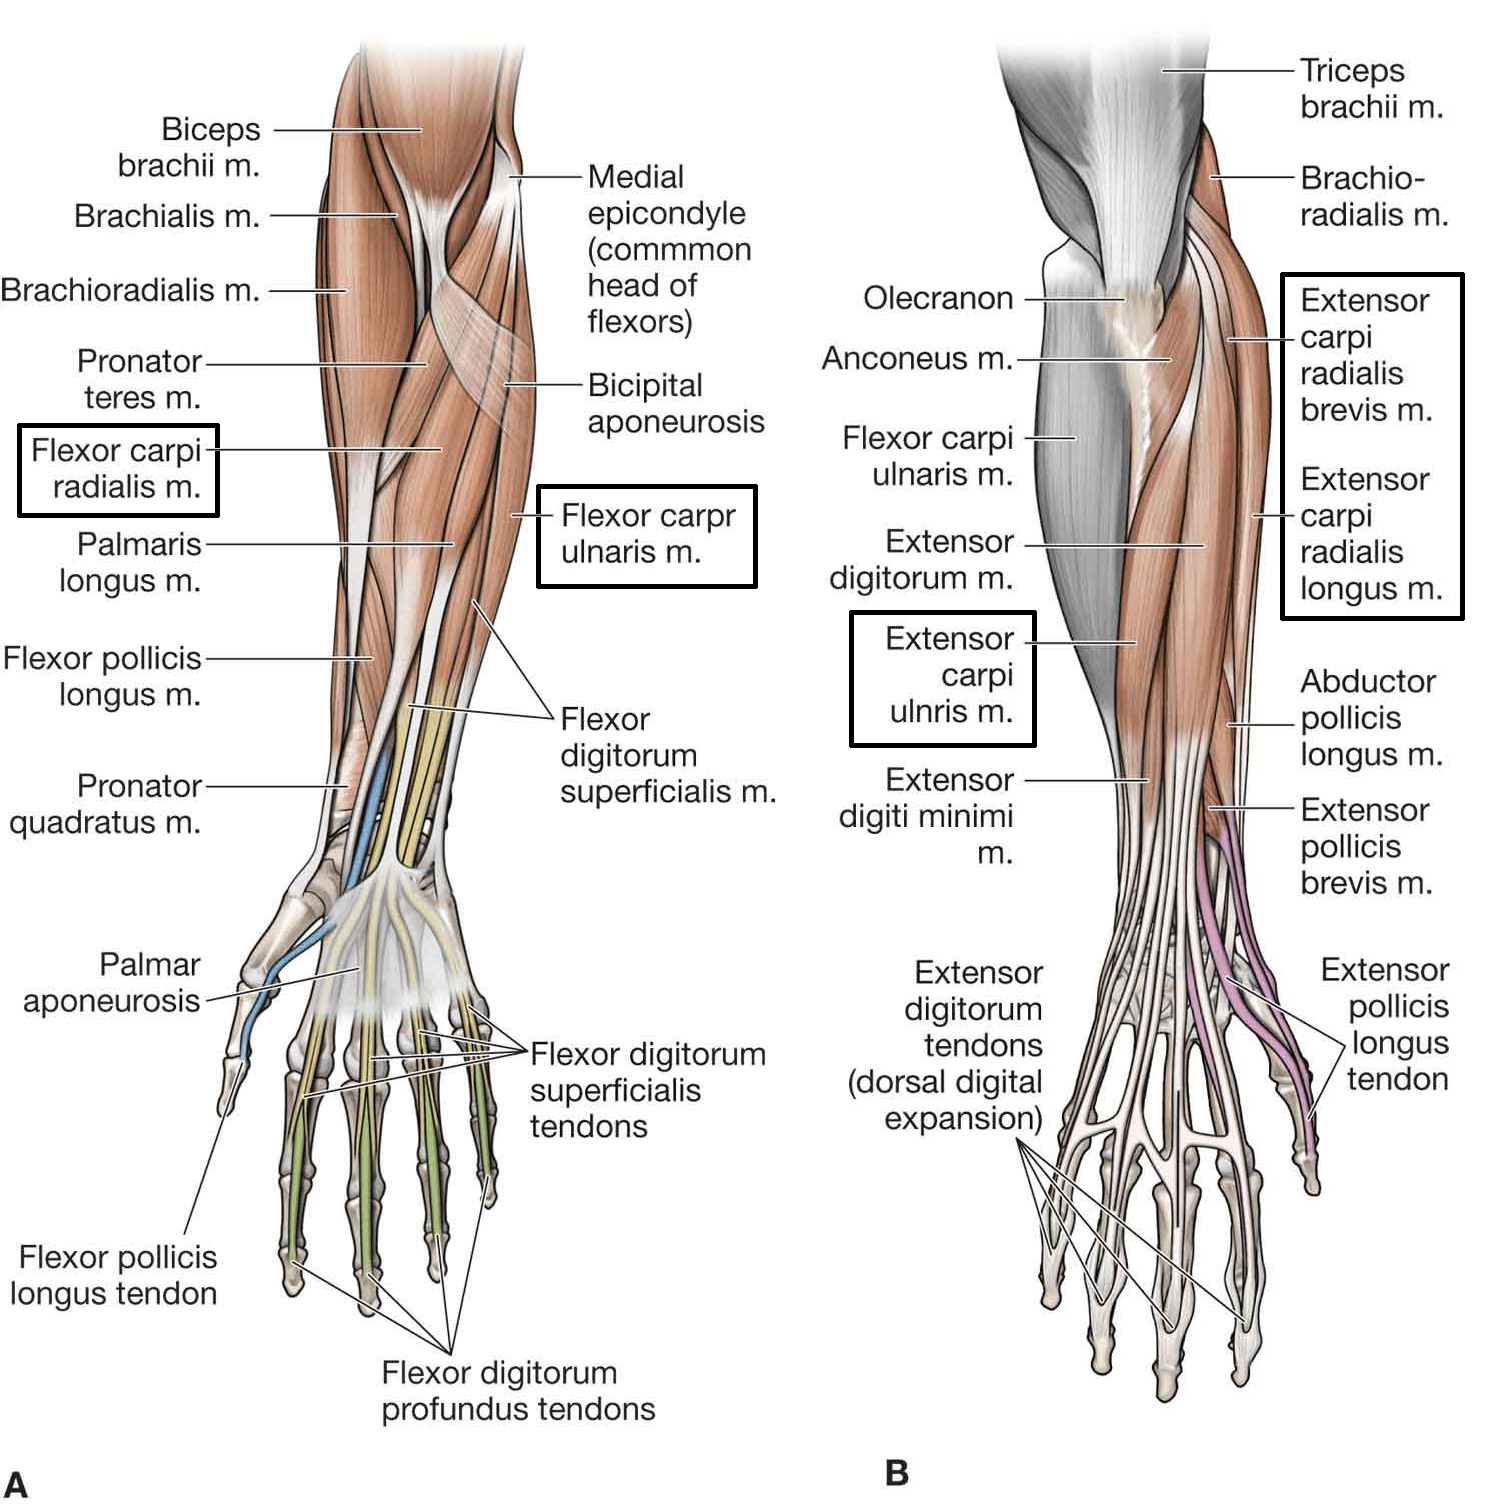
\includegraphics[width=0.7\textwidth]{figures/xBackground/aAnatomy/lowerArm}
%%	\caption{\textbf{A)} anterior view of lower muscles. \textbf{B)} posterior view of lower muscles. The boxed names are of muscles included in both flexion/extension and ulnar/radial deviation. \cite{7semesterprojekt}}
%%	\label{fig:lowerArm}
%%\end{figure}
%
%
%
%

\section{Electromyography} \label{sec:BG:EMG}

This project will utilize the method of electromyography to record the muscle activation of the lower arm muscles in relation to the movements presented in \secref{sec:BG:anatomy}. To develop theoretical background knowledge, a short introduction of the essentials of the signal will be presented. 

Electromyography is the recording of muscle activation. The amount of activity is found by measuring the electric potential, an action potential triggering a muscle contraction. The process of planning and executing a voluntary movement starts at the motor cortex in the brain, where a nerve impulse is send and travels through the spinal cord to the lower motor neuron. As seen in \figref{fig:motor} the path from alpha motor neuron through the axon to the motor endplates is what makes up a motor unit. The alpha motor neuron originates from the spinal cord along the axon to the muscle it controls. The axon branches out to multiple muscle fibers through motor endplates innervating the muscle fibers.
%Muscle movement demanding high precision have a higher innervation of motor units than muscles used for more powerful movements. 

\begin{figure}[H]                                         
	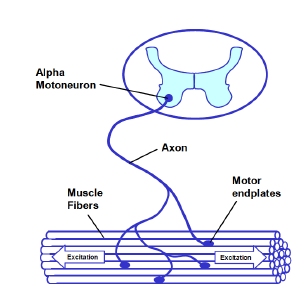
\includegraphics[width=.4\textwidth]{figures/motor_unit}  
	\caption{The figure illustrates the neural pathway from the alpha motor neuron to the innervated muscle fibers, making up a motor unit. \cite{Konrad2005}}
	\label{fig:motor} 
\end{figure}  

%The essentials of understanding the application EMG is the excitation of muscle cells. The excitability of the muscle fibers play a crucial role in a muscle contraction. The mechanisms of a contraction can be understood through a series of events. First the muscle cell membrane is at a resting potential between -80 to -90 mV, due to an equilibrium of NA$^+$ and K$^+$ through the intracellular and extracellular side of the membrane, maintained by an ion pump. The before mentioned alpha motor neuron reaches the motor endplates where a transmitter substance is released. The substance alters the membrane characteristics and allows a greater flow of Na$^+$ into the cell. This causes a membrane depolarization, changing the membrane potential. If a threshold between -55 mV to -50 mV is reached excitation in the form of an action potential is formed, travelling in both directions of the muscle fiber, as seen on \figref{fig:motor}. The membrane potential is quickly restored with a great outflow of Na$^+$, resulting in a repolarization. 

A fundamental part in the application of EMG is the understanding of the excitation of muscles. Muscles contract through a series of steps of changing potentials across muscle cell membranes and rapid polarization and repolarization. However, when recording EMG it is the superposition of the spread of the motor unit action potentials (MUAPs) over the muscle membrane that is recorded. \cite{Cram2012} 
Muscles are innervated by a varying number of nerves depending on the individual muscle. The MUAP is conducted to the muscle by nerves from the spinal cord, with the nerve impulses originating from the motor cortex in the brain. Muscles are not activated randomly by individual nerve fibers, but by nerves sorted into motor units. Many motor units are attached to a muscle and consist of a number of the nerves innervating the muscle. An illustration of how one motor unit attach to the muscle fibers of a muscle is illustrated in \figref{fig:motor}. When a motor unit activate, all the nerves in the motor unit is activated. This enables a controlled activation of the muscle as well as a activation that reach a higher number of muscle fibers. Motor units are also activated in an asynchronous pattern which enables different muscle fibers to be active at different times, making muscles less prone to fatigue. %The action potential from each of the activated muscle fibers summates spatially and temporally forming a motor unit action potential (MUAP). The spread of the MUAP over the muscle membrane is recorded with EMG.Regulating the number of recruited motor units is a way of controlling the force of a muscle contraction depended on the force needed. The frequency of motor unit activation can also be modulated for generating a specific amount of force. However, as different muscles recruit and activate muscle fibers at different frequencies, the amplitude and frequency visible from an EMG recording is necessary correlated with the generated muscle force. 
The force of a muscle contraction can be modulated either by motor unit recruitment or be frequency of activation. In EMG it is the sum of activity of activate motor units that is recorded. \cite{Cram2012}

In the scenario of this project multiple EMG electrodes will record signals from many muscles in the lower forearm. This will result in some muscles being active during some movements as they contract, while other muscles will be inactive. On an EMG recording this will be visible as contracting muscles will show high activity, while others will show little to no activity. An illustration of this can be seen on \figref{fig:EMGactivityExtensionFlexion}. The figure shows the muscle activity of muscles in the forearm when performing first extension at the wrist followed by flexion. As can be seen the muscle activity is very different between the two muscles. This enables the recognition of specific movements based on several EMG recordings with several different electrode placements. 
%The number of motor units innervating muscle fibers depend on the muscle characteristics and the purpose is serves. A low innervation ratio between motor units and muscle fibers gives the opportunity of fine motor tasks, while a low ratio is ideal for tasks demanding strength. Furthermore the motor units are recruited in an asynchronous pattern. This further facilitates the possibility of smooth muscle movements. \cite{Martini2012, Cram2012}

\begin{figure}[H] 
	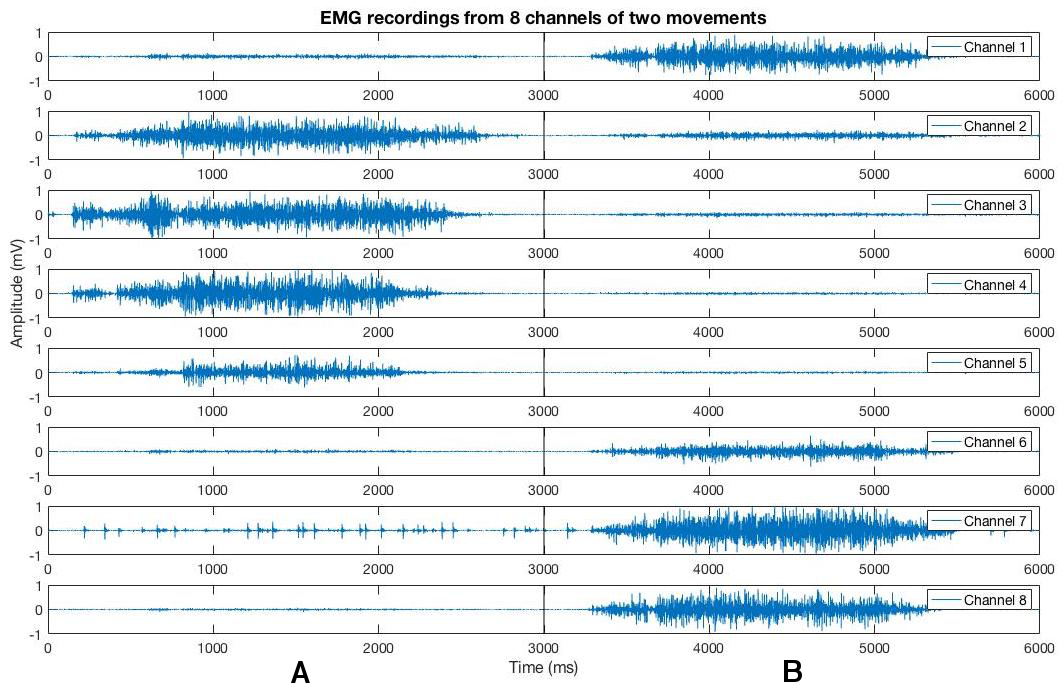
\includegraphics[width=0.9\textwidth]{figures/xBackground/EMGactivityExtensionFlexion}
	\caption{Illustration of the activity in an EMG recording of two movements: extension and flexion. Left side A) shows the activity recorded by EMG electrode channels during extension of the hand. Right side B) shows activity during flexion of the hand.}
	\label{fig:EMGactivityExtensionFlexion}
\end{figure}


Recording EMG can be done either through the most often used surface EMG (sEMG) or by intramuscular EMG (iEMG). In iEMG a needle is inserted into the muscle measuring the MUAP directly on site. The more often used sEMG that uses electrodes to measure the sum of MUAPs on the skin surface, will be used to acquire EMG signals in this project. \cite{Cram2012}





As presented earlier in \fxnote{ref to emg} the source of sEMG signal is the motor unit action potentials. The energy generated in action potentials is of a very small size and is measured in microvolts. Very sensitive recording equipments is therefore key in doing electromyography. Essential is to consider the type of electrode intended to use. Electrodes come in varies different sizes and shapes and are therefore very depended on the intended measurement site. Typically are electrodes made of silver-impregnated plastic used. They present desired characteristics by being disposable, relatively low price and by having low impedance with the skin. Most electrodes are covered with some adhesive compound in order form them to stick to the skin. These can either be 'dry' or covered with different types of gel, in order to reduce impedance and thereby noise, getting a more accurate EMG recording. Dry electrodes do not use gel, but instead rely on the skin to sweat thereby decreasing the skin impedance. Dry electrodes should prove better to patients with sensitive skin.\cite{Cram2012} Different skin conditions may also effect the electrode-skin impedance. People with makeup, scale or much hair increases the impedance, why the site should be shaved or rinsed with an alcoholic wipe.   




 



\section{Myo armband overview} \label{sec:MYB}

The Myo armband (MYB) from Thalmic Labs will be used for EMG data acquisition. It contains eight dry stainless steel electrode-pairs around the inside of the armband, as depicted in \figref{fig:myoarmband}. The recorded EMG is unitless in an 8-bit resolution. As usual when recording EMG the higher the performed contraction is, the higher the integer values in the output will be. To avoid interference from power lines a 50 Hz notch filter is implemented in the MYB. However, the MYB is not able to make any further filtering, thus this will be implemented later during signal processing described further in \secref{sec:prePros}. The MYB has a 200 Hz sample rate. Besides the EMG sensors the MYB can provide position and orientation information, using its three inertial measurement units consisting of a three axis gyroscope, a three axis magnetometer and a three axis accelerometer. This inertial information is sampled at 50 Hz. \cite{Myoarmband2013}

\begin{figure}[H]                 
	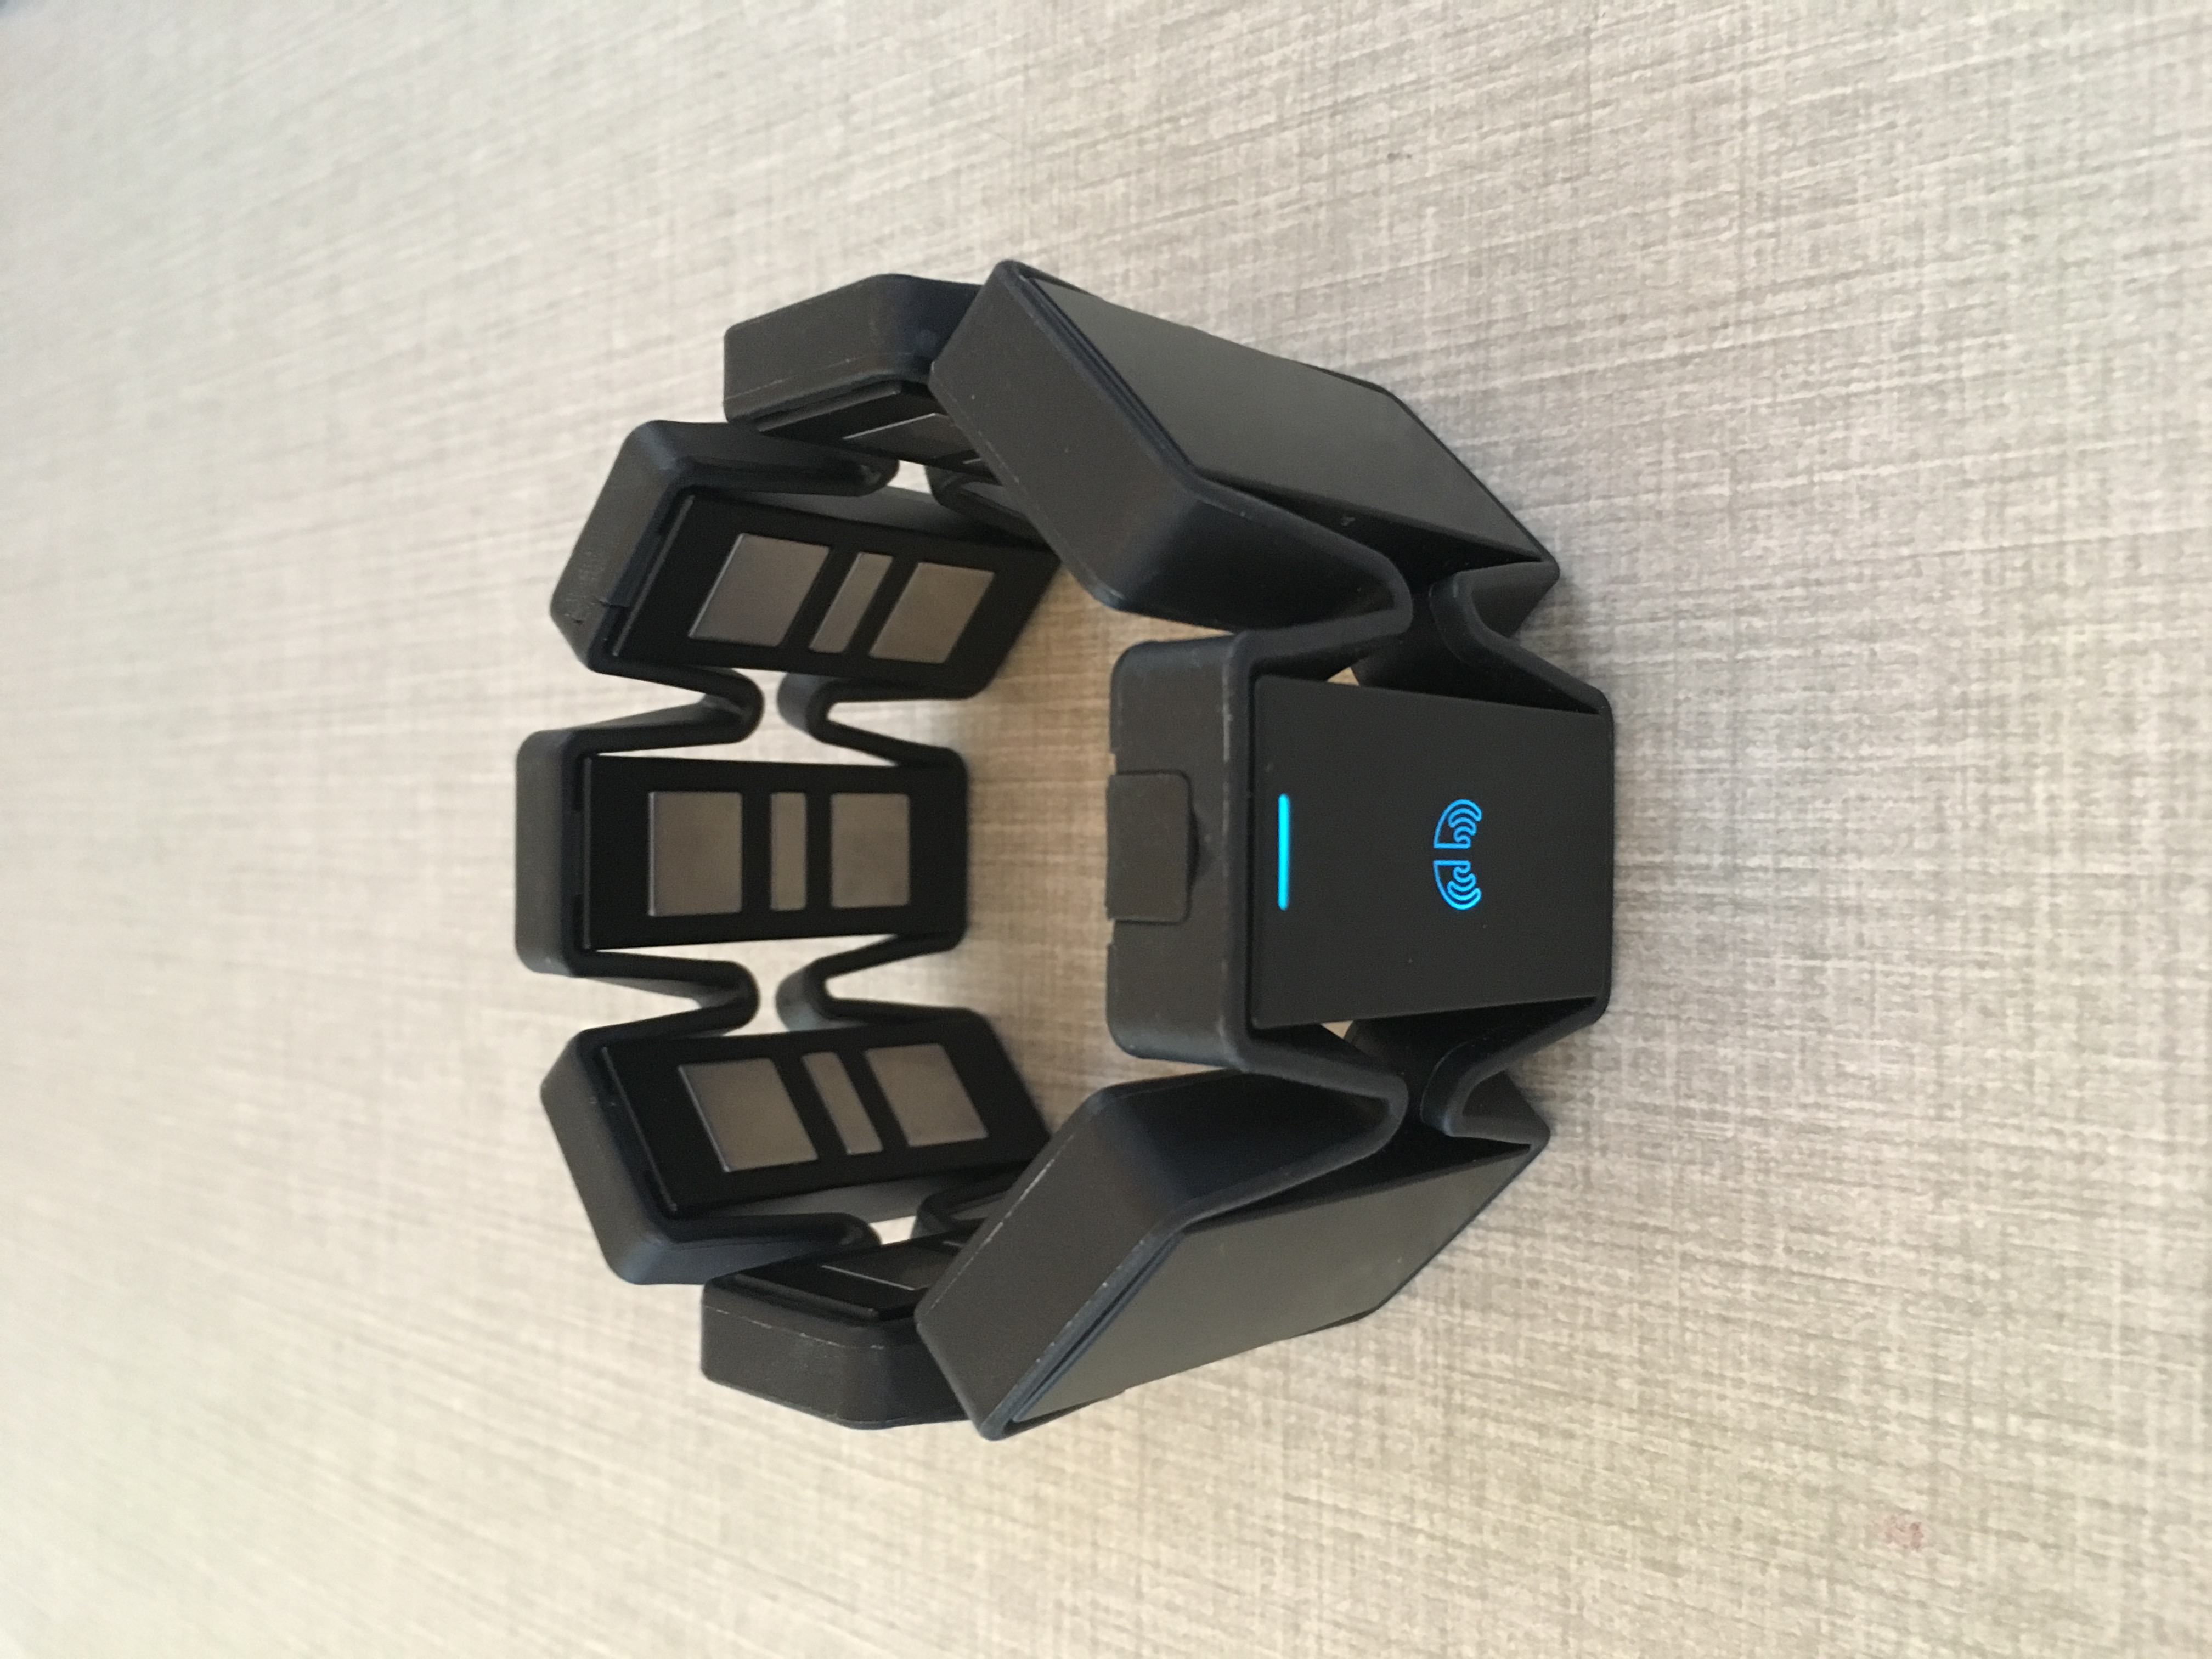
\includegraphics[width=.4\textwidth]{figures/xBackground/myoband}  
	\caption{Myo armband from Thalmic Labs.}
	\label{fig:myoarmband} 
\end{figure}

When initiating the wearing of the armband there is two calibration phases the user must follow before the armband is ready to use - the warm-up phase and the sync phase. During the warm-up phase the armband is ensuring a strong electrical connection with the muscles in the forearm as possible. This is mainly provided by light sweating on the skin under the electrodes, which improve the connection similar to electrode gel \cite{Cram2012}. During the sync phase, the armband determines its orientation in space, position on and which arm it is placed on. The MYB works better when fitted tightly on the thickest part of the forearm. For users with smaller forearms a set of clips can be added to the armband to get a constrained grip. \cite{Myoarmband2013}

\section{Data processing} \label{sec:pross}


In order to use the acquired EMG-signal in myoelectric prosthesis control, it first has to be processed, this is also refereed to as pre-processing. Since the acquisition and most processing is done in the MYB before Bluetooth transmission, further processing of the signal before use is kept at a minimum. In myoelectric prosthesis control features are extracted for use in control, instead of using the entire EMG-signal. Hereby the amount of information is reduced resulting in faster computational speed by reducing redundant information. The following two sections will briefly describe theory behind filtering and feature extraction in relation to this project.  


\subsection{Filtering} \label{sec:filt}

Filtering is a cornerstone in preparing an EMG-signal for any kind of use. The frequency spectrum of EMG is 10 Hz to 500 Hz and most electrodes has a working range of 0 Hz to 500 Hz \cite{DeLuca2010}. According to the Nyquist theorem, to achieve a loss-less representation of the signal the sampling frequency must be at least twice the maximum frequency of interest of the original signal \cite{Pozzo2004}. Besides sampling with twice the maximum frequency, EMG is sensitive to artifacts of movement and electrical interference. Due to these circumstances, filters are often implemented to remove these unwanted contributers \cite{DeLuca2010}. 
General practice in filtering the EMG-signal will imply implementing a notch filter with very narrow width (49-51 Hz) or (59-61 Hz) depending on the power supply and with a very steep slope. The intend is to remove any electrical interference noise. In the low frequency spectrum several recommendations (5 Hz, 10 Hz and 20 Hz) has been made for optimal corner frequency of a high pass filter, to remove noise. A low pass filter is also introduced to remove any noise and unwanted signal above 500 Hz \cite{Cram2012}. 

This project will utilize the MYB for data acquisition and as mentioned in \secref{sec:MYB} the MYB has a sample rate of 200 Hz. In relation to this paper a sampling frequency of at least twice the maximum of the recorded signal is not possible, since muscles of the forearm have a maximum frequency of 400-500 Hz \cite{Cram2012}. This would require a sample rate of at least 1000 Hz, which cannot be achieved due to limitations in the MYB. The effect of the low sample rate of the MYB is aliasing in the recording, causing a frequency component not originally in the EMG signal. To account for this it would be resourceful to implement an anti-aliasing filter.  

\subsection{Feature extraction} \label{sec:fe}

The raw EMG-signal is not itself used for myoelectric prosthesis control, but features that are extracted from it. Thereby reducing the amount of redundant information limiting it to its most useful properties, resulting in faster computational speed. 
There are numerous feature components from an EMG signal which can be extracted either from the time-domain, frequency-domain, or time-frequency domain. Most used are features from the time- and frequency-domain. Time-domain features can be categorized in five different types based on their mathematical properties: energy information complexity information, frequency information, prediction modelling and time-dependency. Extracting features from the frequency-domain requires a frequency transformation, calculating the spectral properties of the recorded signal, which takes up longer processing time than simply using time-domain features. 
Time-domain features are often chosen based on their quick and easy implementation. They do not require any transformation before extraction and are calculated based on the raw EMG-signal. In addition, it is important not to choose redundant features for the classifier; features containing similar information. \cite{Phiny2012} 

Extracting features for real-time prosthesis control are done by taking segments of the continuous signal, called windows, and calculation are therefore done on these discriminated windows. This is done instead of using the instantaneous value due to the signals random nature. These windows are overlapped to create a dense information stream for extraction. The relationship between window and overlap length is significant, when trying to determine the best representation. The window length is a matter of getting enough samples to do the calculation, but to long a window will result in delays slowing the control. Overlapping the window is a way to faster acquire windows by reusing a determined last segment of the prior window. Smith et al. found that the optimal window length that enables best performance ranges from 150-250 ms, in a classification control scheme. \cite{Smith2014} 

\section{Linear Discriminant Analysis}

Linear discriminant analysis(LDA) is a supervised classification method used to separate classes of data by linear decision boundaries. Each decision boundary is a hyperplane $H$ from which the minimum distance from the classes it separates is maximized, and the distance from the means of the classes are maximized. A decision boundary is defined as a linear combination of the feature values x and is given as:

\begin{equation}
g(x) = w^tx +w_0
\end{equation}

where $w$ is a weight vector deciding the orientation of $H$, and $w_0$ is a bias deciding the position of the hyperplane in relation to the origin. In a two category case the decision rule for deciding class $w_1$ or $w_2$ is: decide $w_1$ if $g(x) > 0$ and $w_2$ if $g(x) < 0$. $g(x) = 0$ then defines the decision boundary that separates the features into two decision regions $R_1$ for $w_1$ $R_2$ for $w_2$. $w$ is normal (orthogonal) to any vector on $H$, which can be used to calculate the distance $r$ from feature values to the decision boundary:

\begin{equation}
r = \frac{g(x)}{||w||}
\end{equation} 

From origin the distance is given as $\frac{w_0}{||w||}$, where if $w_0 > 0$ the origin is on the positive side of the decision surface, and if $w_0 < 0$ the origin is on the negative side. In the case of $w_0 = 0$ the decision surface passes through origin. In \figref{geolda} a geometric illustration of the linear discriminant function and its properties  is depicted.

\begin{figure}[H]                 
	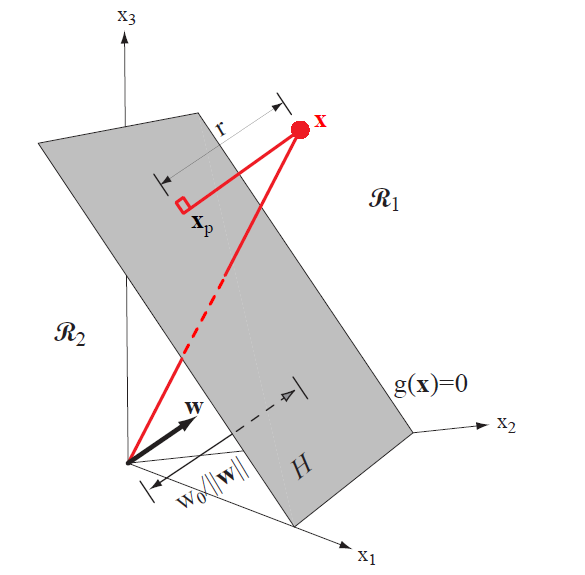
\includegraphics[width=.4\textwidth]{figures/xBackground/geolda}  
	\caption{A geometric illustration of the linear decision surface $g(x)$ that separates the feature space into two decision regions $R_1$ and $R_2$. \cite{Duda2000}}
	\label{fig:geolda} 
\end{figure}

In a multicategory case $c$ decision boundaries are defined. The approach for defining the decision boundaries is given as:

\begin{equation}
	g_{i}(x) = w^tx_i +w_{i0} ~~~~~~~~~~~ i = 1,...,c,
\end{equation}

where $x$ is assigned to $w_i$ if $g_i(x) > g_i(x)$ for all $j \neq i$. This type of classifier is called a linear machine, and will be adopted as classification method in this project. 


%background regression 
\section{Linear regression methods}
Classification can be used together with regression methods to provide a combination of the two control scheme. The output from the LDA classifier can be set to only decide on which movement is performed, and not
%The output from the LDA classifier only decides on which movement that is performed, and not 
at which contraction level the muscles used in the given movement are performing. Thus, the prosthesis can not perform any movement.  In statistics linear regression is often used to determine relations between variables. This notion can also be applied for myoelectric prosthetic control. While classification only provides an output on which class is recognized, a linear regression model provides a continuous output value based on the input value. If the regression model is fitted with information on different contraction levels for a given movement, control proportional to the contraction level will be achieved \cite{Hwang2017, Hahne2014, Bruun2017}. In the overall control scheme the classifier can then be used to decide which movement is performed, and a regression model can decide at which contraction level the movement is performed at. Similarly as with the classifier, regressors needs to be trained based on data acquired from the user, where the features extracted from the raw EMG signal is used as input. This procedure is described in the following section. 
%The use of linear regression is often used in statistics to determine relations between variables. Regressions methods also has its use in control schemes of myoelectric prosthetics \cite{Hwang2017, Bruun2017, Hahne2014}. The difference between classification and regression is that classification attempt to classify similar patterns in recordings, between previously acquired data and new data, while regression methods provide a continuous output value based on the input value \cite{Mendez2017, Hahne2014}. %\fxnote{sidste sætning er taget fra indtroduktionen men det stykke skal nok skrives om/væk alligevel for det omhandler classifikation VS regression. edit: er taget ud af introduktionen nu.}

Different models of linear regression exist to account for different uses. When utilizing regression methods it must be considered which type of input variables are used and what type of relation these variables might have. The appropriate regression must then be applied. Simple linear regression approximate a relation between one dependent variable $Y$ and one independent variable $X$ \cite{Zar2009}:

\begin{equation} \label{eq:simpleLinearRegression}
Y = \alpha + \beta X + \epsilon
\end{equation}

where $Y$ is the control output for the prosthesis, $X$ is the feature extracted from the EMG signal, $\beta$ is the regression coefficient in the sampled population, $\epsilon$ is the error, and $\alpha$ is the predicted value of $Y$ at $X = 0$.
This model can be expanded to estimate relations between one dependent variable and several independent variables. This is called multivariate regression and expands on the equation of simple linear regression, given in \eqref{eq:simpleLinearRegression} \cite{Zar2009}:

\begin{equation} \label{eq:multiLinearRegression}
\hat{Y} = \alpha + \beta_1 X_{1} + \beta_2 X_{2} + ... + \beta_i X_{i} + \epsilon_i
\end{equation} 

where $i$ in this project would correspond to the number of channels in the MYB \cite{Zar2009}. Since this regression model approximates the relation between several independent variables and one dependent variable, this model can be used as a control scheme in myoelectric prosthetics, and . Here the channel-recordings of muscle activity can be considered independent variables, and used to estimate one control output, which would be the dependent variable. \cite{Bruun2017}



\section{Validating Performance} \label{sec:BG:validatingPerformance}

Measuring the performance of achieved prosthetic control cannot be seen as a trivial task, and different approaches can be used. The achieved performance can be measured by affixing a prosthesis on to the test subject and validate performance hereby. Often, like the current project, the subjects do not consist of actual amputees but instead healthy subject. In these cases, the performance validation is done by implementing a virtual test environment where the subjects is to control an object on the computer screen by performing movements. The following section will further elucidate the procedures of such a virtual test for validating prosthetic control.      


\subsection{Modified Fitts' Law} \label{sub:BG:fitts}

Fitts' Law test is a common method of quantifying performance of movements, first proposed by Paul M. Fitts in 1954 \cite{Fitts1954}. Fitts' Law states the that time required to reach a targeted area is a function of the width and distance of the target. The output of a Fitts' Law test is the throughput, as given by \eqref{eq:TP}. This measure gives an idea of the trade-off between speed and accuracy. A modified Fitts' Law test designed for a virtual 2D and 3D target acquisition test has later been used by \cite{Kamavuako2014} and \cite{Scheme2013} respectively. Here, four additional metrics were added in an real-time test, where a virtual computer cursor was used to represent the control output \cite{Scheme2013, Kamavuako2014}. The four additional metrics, path efficiency, overshoot, stopping distance and completion rate, were made by \cite{Poulton2013} and \cite{Simon2011}. While the throughput measure from the conventional Fitts' Law test is usable, it does not cover all aspects of the control required to complete a test. The additional four measures were added to quantitatively assess performance of naturalness, spontaneity, and compensatory motions during use. The total five proposed performance measures in assessing myoelectric control are \cite{Scheme2013a}: 

Throughput (TP) which represents the trade-off between speed and accuracy. TP uses the relationship of time taken to reach a certain target in seconds ($MT$) and the index of difficulty (ID). This forms: \cite{Scheme2013,Fitts1954}

\begin{equation} \label{eq:TP}
TP=\frac{1}{N}\sum_{i=1}^{N} \frac{ID_i}{MT_i} 
\end{equation}

where $i$ is a specific movement and $N$ is the total number of movements. ID relates to the target distance $D$ and width $W$. The ID for each target, from the origin to a specific target of a certain size is calculated using \cite{Scheme2013,Fitts1954}:

\begin{equation} \label{eq:ID}
ID=log_2(\frac{D}{W}+1)
\end{equation}

Path Efficiency (PE) describes the quality of control by making a measure of the straightness of the cursor's path to the target, by making a ratio of the actual path distance versus the optimal path distance. This tests the users' ability to continuously control the cursor position. Following the optimal path will result in a PE of 100\%. PE is calculated as follows \cite{Scheme2013, Poulton2013}:       

\begin{equation} \label{eq:PE}
PE = \frac{Optimal ~ Distance}{Actual ~ Distance}
\end{equation}		 

Overshoot (OS) is the number of times the cursor enters and then leaves the target before the dwell time inside the target is reached, across all target in the test, divided by the total number of targets. OS tests the users ability to control the velocity of the cursor accurately. A perfect OS-score of zero is reached if the cursor dwells within the target boundaries on the first try for all targets, and is calculated as the following \cite{Scheme2013, Poulton2013}:

\begin{equation} \label{eq:OS}
OS = \frac{Total ~ Number ~ of ~ Overshoots}{Total ~ Number ~ of ~ Targets}
\end{equation}

Stopping Distance (SD) describes the users ability to rest and thereby perform no movement. The SD measure is the distance moved during the dwell time across all targets, and is given as \cite{Scheme2013}:

\begin{equation} \label{eq:SD}
SD = \sum_{i=1}^{N} (Distance ~ Inside ~ Target)_i
\end{equation}

where $i$ is a reached target and $N$ is the total number of reached targets.

Completion Rate (CR) describes the percentage of targets reached within the total allowed time. This gives a general idea of the user's performance, and is calculated as \cite{Scheme2013,Simon2011}: 

\begin{equation} \label{eq:CR}
CR = \frac{Number ~ of ~ Reached ~ Targets}{Total ~ Number ~ of ~ Targets}
\end{equation}




\chapter{Methods}

%\section{Study Design}

\begin{figure}[H]                                         
	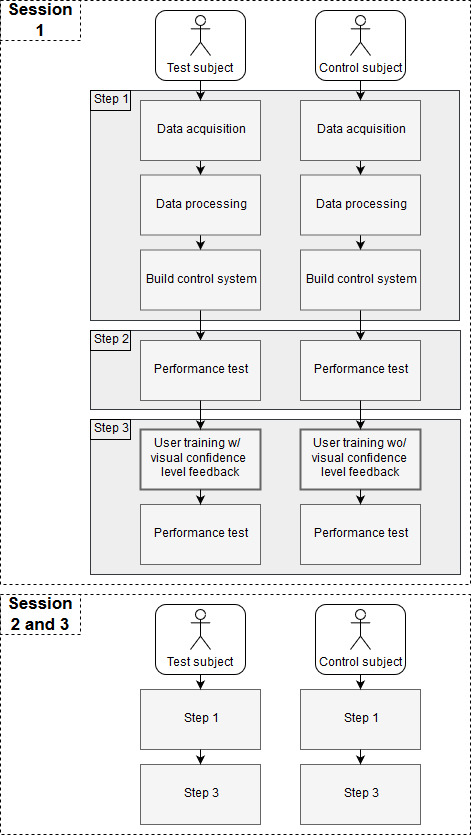
\includegraphics[width=.64\textwidth]{figures/pMethods/Study_design}  
	\caption{Ttext}
	\label{fig:motor} 
\end{figure}  
%data acquisition
\section{Data Acquisition} \label{sec:M:dataAcquisition}

This section will clarify the method of acquiring data in this project. For data acquisition the MYB was used to record EMG signals from muscles in the forearm. The recordings were made on test subjects instructed to perform six different hand movements as introduced in \secref{sec:BG:anatomy}. 


%As described in \secref{sec:MYB} about the MYB, the armband has a sample rate of 200 Hz. 
%According to the Nyquist theorem, to achieve a loss-less representation of the signal the sampling frequency must be at least twice the maximum frequency of interest of the original signal \cite{Pozzo2004}. In relation to this paper a sampling frequency of at least twice the maximum of the recorded signal is not possible, since muscles of the forearm have a maximum frequency of 400-500 Hz \cite{Cram2012}. This would require a sample rate of at least 1000 Hz, which cannot be achieved due to limitations in the MYB. The effect of the low sample rate of the MYB is aliasing in the recording, causing a frequency component not originally in the EMG signal. To account for this an \textbf{anti-aliasing filter is implemented}, described further in \secref{sec:prePros} on preprocessing of the signal. Thus, data will be acquired as a sampling frequency of 200 Hz.

For acquiring data a Graphical User Interface (GUI) was designed. In the GUI the possibility to change settings for different types of recordings was implemented. The first type of recording was a baseline measurement. This recording was made in order to be able to reduce the baseline noise. This was done by subtracting the baseline from the EMG signal when the the EMG signal reached higher than the baseline. When the EMG signal was below the baseline, it was set as 0. \\
The second recording type was a Maximum Voluntary Contraction (MVC) which was a 15 second recording of the subject's maximum contraction of one movement that could be kept constant for 15 seconds without developing muscle fatigue. The mean MVC across all channels was set as a reference value for the following recordings. \\
The third type of recording was of EMG signals used to train the control system. The recordings of EMG signals were based on fractions of the MVC, which could be set using a menu in the GUI. As stated in \secref{sec:M:usertraining}, three contraction levels was used: 40\%, 50\% and 70\%. The level of contraction defined the height of the plateau of a trapezoid trajectory which would be plotted in a window in the GUI. When doing EMG recordings the subjects must perform the instructed movement to control the height of a cursor in the trapezoid plot to best match the trajectory of the trapezoid. The cursor height was calculated as the mean EMG signal across channels normalized based on the MVC. The subject only controlled the height (EMG intensity) of the cursor as the cursor would automatically move forward along the x-axis in relation with time. The recording time was 15 seconds: 2.5 seconds rest at the initiation and ending, 2.5 seconds on the trajectory incline and decline and 5 seconds on the plateau. Of the recorded time only the plateau phase and the last second of the incline and first second of the decline were used to fit the classifier. This approach provided data from a performed movement in both the transition and steady state phase. This data acquisition method was applied since the use of dynamically changing force data in training a classification-based control scheme has shown to improve performance and tolerance to proportional control \cite{Scheme2015}. 
During recordings the investigators evaluated whether the subject followed the trajectory well enough. Furthermore to evaluate the training data, the investigators observed a spider-plot during the acquisition, which was seen on the right side in the GUI. The spider-plot showed the amplitude output for each channel in the MYB. If the activation pattern of the channels changed dramatically, it was a sign of fluctuations in muscle activation, and thus the subject did not perform the instructed movement. If this was observed the recording was discarded and a new was be acquired. An illustration of the data acquisition GUI is shown in \figref{fig:GUIplot}.

\begin{figure}[H] 
	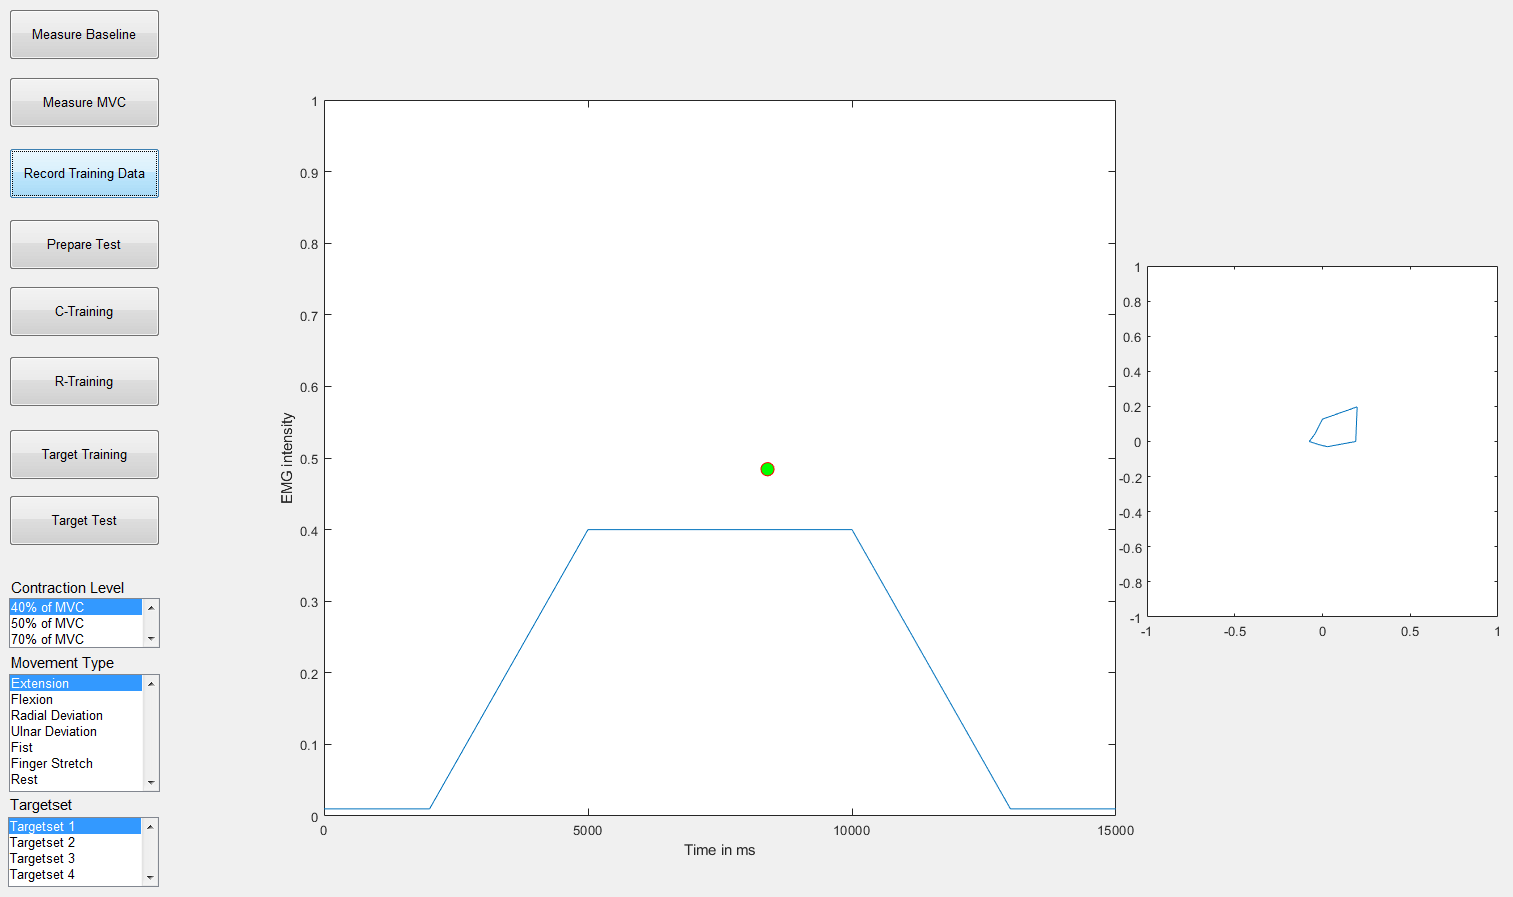
\includegraphics[width=1\textwidth]{figures/xBackground/dataacqGUI}
	\caption{The implemented data acquisition interface. On the left is different buttons shown, where only "Measure Baseline", "Measure MVC" and "Record Training Data" is used in the data acquisition. The "Contraction Level" menu forms the trapezoidal trajectory and "Movement Type" saves the performed movement the correct label. In the center is the trapezoidal trajectory and the cursor representing the EMG signal. On the right is the spider-plot used to evaluate the quality of the performed movement.}
	\label{fig:GUIplot}
\end{figure}



\section{Data processing}

The following two sections will cover the implementation of the filter used to prepare the EMG-signal and the extraction of features to represent the signal. Choices behind implemented methods builds on background knowledge acquired in \secref{sec:pross}. 


\subsection{Filtering of signal} \label{sec:prePros} 

As earlier mentioned in \secref{sec:filt}, due to the MYB specifications limiting the sample rate to 200 Hz and movement artefact's in the low-frequency spectrum, it would be resourceful to implement a bandpass filter to avoid a biased signal.
In the interest of representing the signal with its true properties a second order Butterworth bandpass filter has been implemented with cut-off frequencies of 10 Hz and 90 Hz. A filter steeper than second order was deselected due to a chosen trade-off between filter performance and computational performance, which is of great importance when doing real-time control. Below in \figref{fig:filt} is the result of implementing the bandpass filter shown. The unfiltered signal (top) shows frequency components in low-frequency spectrum around 0-10 Hz and indicating frequency components above above 100 Hz. Both ends of the spectrum has been dampened limiting impact of artefact's and possible aliasing. Furthermore is the presence of the build-in 50 Hz notch filter elucidated as explained in \secref{sec:MYB}.     


\begin{figure}[H]                 
	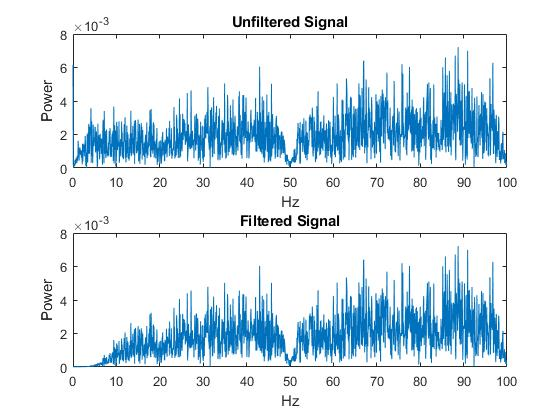
\includegraphics[width=.8\textwidth]{figures/pMethods/Filt}  
	\caption{Output showing the difference before an after implementing the bandpass filter. The unfiltered signal shows frequency components in low-frequency spectrum around 0-10 Hz and indicating frequency components above above 100 Hz. }
	\label{fig:filt} 
\end{figure}





\subsection{Feature extraction}

The features chosen to represent the information of movements contained in the signal is primarily based on recommendations from \cite{Donavan2017} where they found the optimal features for a real-time classification control scheme using the MYB. Donavan et al. used so called space domain features along with the MYB and got a five percent higher accuracy than by using the well known Hudgins time domain features. A total of seven features, Mean Absolute Value (MAV), Mean Mean Absolute Value (MMAV), Scaled Mean Absolute Value (SMAV), Correlation Coefficient (CC), Mean Absolute Difference Normalized (MADN), Mean Absolute Difference Raw (MADR) and Scaled Mean Absolute Difference Raw (SMADR) were derived and the following section will explain the extraction of each. Only SMAV, CC, MADN and SMADR were used for the final classification to reduce redundancy, but all seven will be explained because the some features are a combination of others. \cite{Donavan2017} Furthermore it has been chosen to extract the time domain feature of waveform length (WL) to represent frequency related information of the signal. The extraction of this feature will lastly be explained as well. 

\begin{flalign}
	MAV_i=\frac{\sum_{n=1}^{wl}}{wl}
	\label{TP}
\end{flalign}
      




\begin{flalign}
	MMAV=\frac{\sum_{i=1}^{8}MAV}{8}
	\label{TP}
\end{flalign}




\begin{flalign}
	SMAV_i=\frac{MAV_i}{MMAV}
	\label{TP}
\end{flalign}




\begin{flalign}
	CC_i=\frac{\sum_{n=1}^{wl}X_i[n]X_{i+1}[n]}{\sum_{n=1}^{wl}X_i[n]^2}=\frac{\sum_{n=1}^{wl}X_i[n]X_{i+1}[n]}{wl}
	\label{TP}
\end{flalign}



\begin{flalign}
	MADN_i=\frac{\sum_{n=1}^{wl}|X_i[n]-X_{i+1}[n]|}{\sum_{n=1}^{wl}X_i[n]^2}=\frac{\sum_{n=1}^{wl}|X_i[n]-X_{i+1}[n]|}{wl}
	\label{TP}
\end{flalign}


\begin{flalign}
	MADR_i=\frac{\sum_{n=1}^{wl}|X_i[n]-X_{i+1}[n]|}{wl}
	\label{TP}
\end{flalign}




\begin{flalign}
	SMADR_i=\frac{MADR_i}{MMAV}
	\label{TP}
\end{flalign}
















\section{Experiment protocol} \label{sec:Eprot}

\textbf{Title of project}

Using confidence levels of movement recognition in user training to improve prosthesis control 

\textbf{Detail on investigators}

All investigators are 2th semester biomedical engineering master students at Aalborg University.  

\textbf{Purpose and background}
Electromyography(EMG) is widely used for controlling functional lower arm prosthetics for transradial amputees. The ideal purpose of a functional prosthesis is to behave as functional as possible compared to a biological arm. Functional prosthetics that rely on pattern recognition-based control are becoming exceedingly good in performance in a clinical environment, due to highly optimized system control. However, still only one commercially available pattern recognition-based prosthesis exist. Users reject these functional prosthetics usually due to functionality issues when utilizing them in daily life tasks outside the clinical environment. Many improvements have been made in the area of system control, but another approach of improving the prosthetic control is by training the user. User training has only been explored moderately in the research literature, thus, techniques to improve the user's ability to control a prosthesis are yet untouched. This experiment will focus on training the user to improve prosthetic control on a fixed pattern recognition-based control system. The novel approach in this study is to provide the user with information on how well the system recognizes the performed movement during user training. 

%Commercially available prosthesis have yet to adopt the use of pattern recognition methods in their control scheme. Mainly, this is due to the disadvantages exploited in “ref til introduction om problemer måske?”. A control scheme that reduce these disadvantages are therefore sought through the combination of regression and classification based methods. 
%The overall aim is to develop a novel control scheme for myoelectric prosthetic devices. Hereby it is sought to clarify if a combined regression and classification control scheme yields higher subject performance in a Fitts’ Law test compared to a method only using regression.

\textbf{Research hypothesis}

Exposing subjects to user training, in which confidence levels of movement recognition is used as feedback, will show improvement in performance in a classification-based myoelectric prosthetic control scheme.% across short training sessions. 

\textbf{Ethical considerations}  

The investigators do not foresee any obstacles of ethical nature during the proceedings of this experiment. No test subjects will be exposed to any physical interventions besides being asked to wear the Myo armband. No part of this experiment should put the subject in danger. 

\textbf{Session time} 

The experiment consist of three sessions, which are spread over three consecutive days; one session per day. Each session is estimated to have a total duration of 30-60 minutes. 

\textbf{Inclusion criteria}

The subject needs to be:
\begin{itemize}
	\item able bodied.
	\item between 18 and 60 years of age.
	\item able to understand and speak Danish and/or English.
	\item assessed by the investigators to understand and perform the instructions given during the experiment. 
\end{itemize}


\textbf{Exclusion criteria}

The subject must not have:
\begin{itemize}
	\item diseases that might influence subject performance. 
\end{itemize}


\textbf{\Large{Experiment procedure}}

The experiment consists of three sessions containing different steps as illustrated on \figref{fig:experiment_protocol_pipeline}. The concept and chronology of each step is described below the illustration.


\begin{figure}[H]                                         
	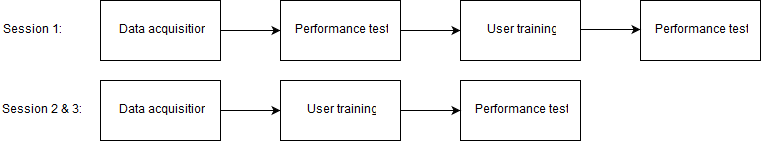
\includegraphics[width=0.9\textwidth]{figures/pMethods/experiment_protocol_pipeline}  
	\caption{Pipeline for the three sessions in the experiment and what steps each session contains.}
	\label{fig:experiment_protocol_pipeline} 
\end{figure}  


\textbf{Data acquisition}

For the myoelectric control system to be able to identify a performed movement as the movement that is actually performed, it needs information about how the movement looks when represented as a EMG signal. Thus, EMG data needs to be acquired from the forearm of the subject meanwhile the subject performs the movements that is used in the experiment, see \figref{fig:experiment_movements} on the last page. This data is fed to the control system for it to be able to recognize each movement. In this experiment EMG data will be acquired from the subject with an EMG-electrode armband: Myo armband(MYB) from Thalmic Labs. The chronology of this step is as follows:

\begin{enumerate}
	\item Apply MYB on dominant forearm at the thickest part.
	\item Synchronize MYB by performing wrist extension until three distinct vibrations are felt.
	\item Perform 15 seconds of maximum voluntary contraction (MVC) of instructed movement. Following the MVC the subject will be given a 15 seconds resting period to avoid muscle fatigue.
	\item Perform three 15 seconds contraction trails of respectively 40\%, 50\% and 60\% of MVC. During these contractions the subject will control a green marker representing the EMG signal and try to follow a trapezoidal trajectory as precise as possible. The trapezoidal trajectory consists of two five second transition phases and one five second plateau phase. Between each trial the subject will be given a 10 seconds resting period to avoid muscle fatigue.
	\item Repeat step 3-4 until training data from all four wrist movements has been recorded.
\end{enumerate}

An illustration of the interface used for data acquisition is shown in \figref{fig:dataacqGUI}

\begin{figure}[H]                 
	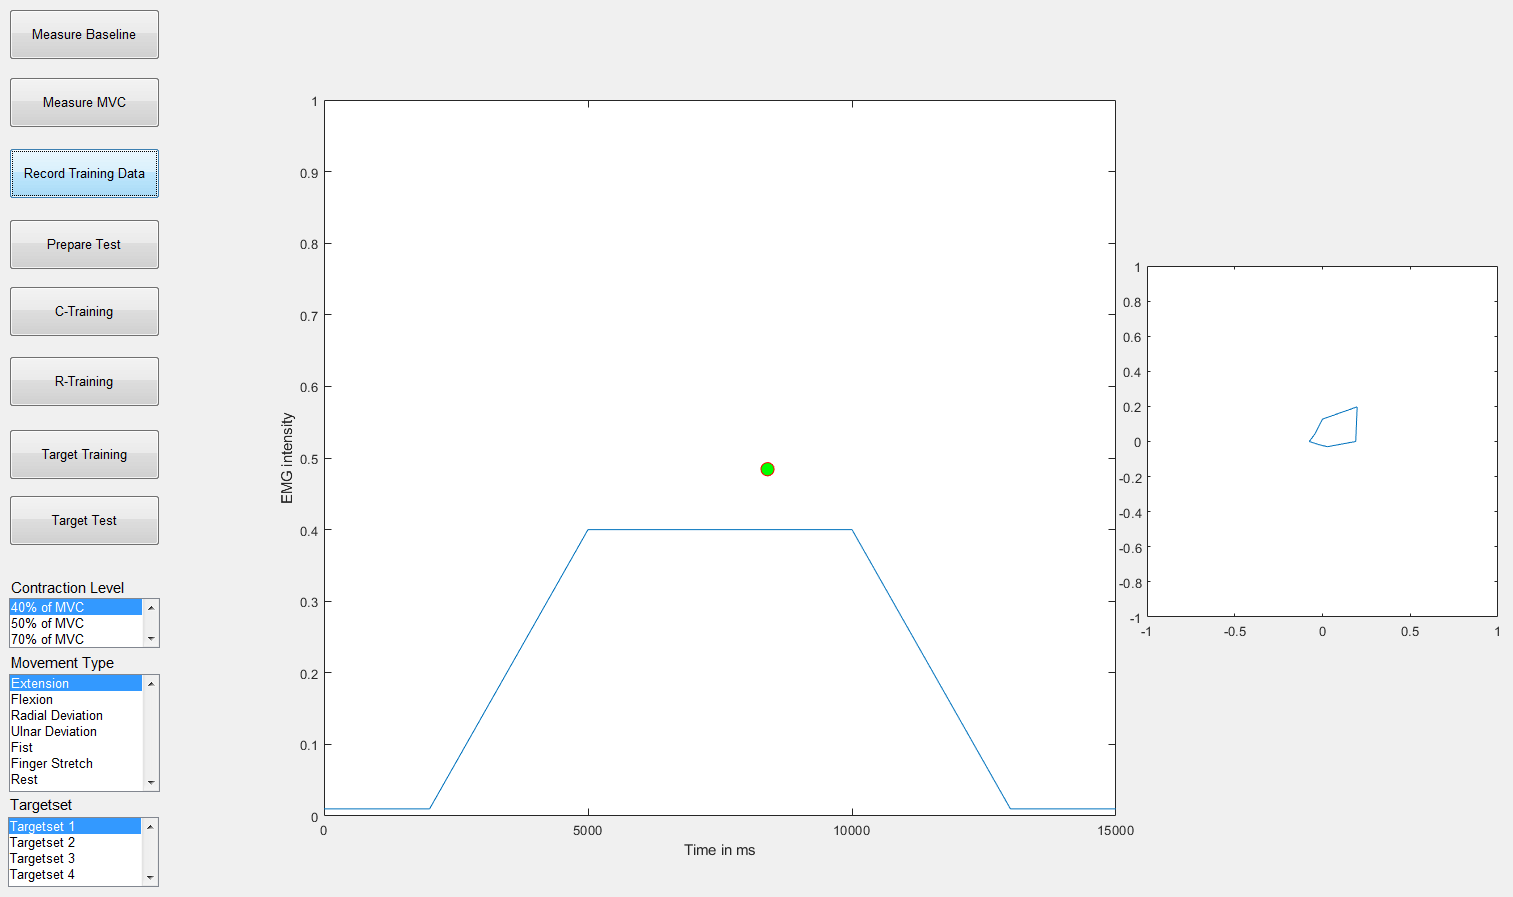
\includegraphics[width=.6\textwidth]{figures/xBackground/dataacqGUI}  
	\caption{Illustration of the data acquisition interface showing the trapezoidal trajectory and the green marker representing the EMG signal.}
	\label{fig:dataacqGUI} 
\end{figure}

\textbf{User training} %test group

The purpose of user training is for the subject to train the movements used in the performance test. During the user training the subject will train one movement at a time in different contraction levels. When training a movement, visual feedback in form of confidence levels on how well the control system recognizes movements, is shown in percentage in a bar plot. In addition, the level of contraction is shown in a text box above the bar plot. When performing the instructed movement at the instructed level of contraction the background colour of the text box will appear green; if it is within the instructed level it appears red. The aim for the subject is to reach and withhold the instructed contraction level with 100 \% recognition certainty for each movement. The chronology of this step is as follows:

\begin{enumerate}
	\item Perform flexion at 15-25 \% contraction level for 20 seconds followed by 10 seconds rest.
	\item Perform extension at 15-25 \% contraction level for 20 seconds followed by 10 seconds rest.
	\item Perform radial deviation at 15-25 \% contraction level for 20 seconds followed by 10 seconds rest.
	\item Perform ulnar deviation at 15-25 \% contraction level for 20 seconds followed by 10 seconds rest.
	\item Perform open hand movement at 15-25 \% contraction level for 20 seconds followed by 10 seconds rest.
	\item Perform closed hand movement at 15-25 \% contraction level for 20 seconds followed by 10 seconds rest.
	%\item Perform instructed movement smoothly increasing the contraction level from 30 \% to 70 \% within x seconds. When reaching the 70 \% contraction level the subject decreases the contraction level to 30 \% within x seconds.
	\item Repeat step 1-6 at 35-45 \% contraction level.
	\item Repeat step 1-6 at 55-65 \% contraction level.
	\item Repeat step 1-6 at 75-85 \% contraction level.
\end{enumerate} 

An illustration of the interface used for user training is shown in \figref{fig:usertraintestGUI}

\begin{figure}[H]                 
	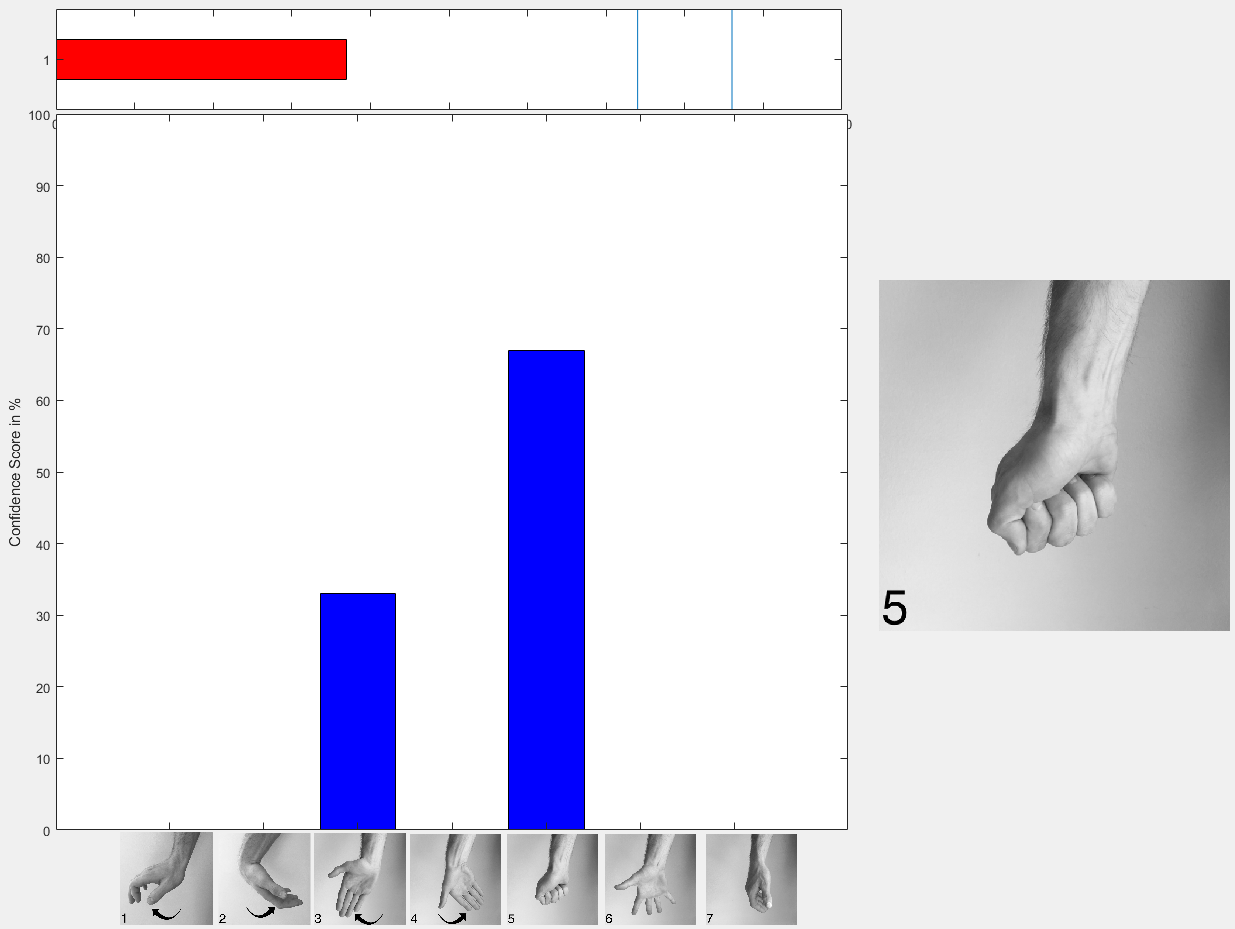
\includegraphics[width=.6\textwidth]{figures/xBackground/usertraintestGUI}  
	\caption{Illustration of the user training interface showing the bar plot indicating the confidence level of movement recognition and the text box indicating contraction level.}
	\label{fig:usertraintestGUI} 
\end{figure}

\textbf{User Training} %control group

The purpose of user training is for the subject to train the movements used in the performance test. During the user training the subject will train one movement at a time in different contraction levels. When training a movement, visual feedback on which movement the control system recognizes, is shown in percentage in a bar plot. In addition, the level of contraction is shown in a text box above the bar plot. When performing the instructed movement at the instructed level of contraction the background colour of the text box will appear green; if it is within the instructed level it appears red. The aim for the subject is to reach and withhold the instructed contraction level with 100 \% recognition certainty for each movement. The chronology of this step is as follows:

\begin{enumerate}
	\item Perform extension at 15-25 \% contraction level for 20 seconds followed by 10 seconds rest.
	\item Perform flexion at 15-25 \% contraction level for 20 seconds followed by 10 seconds rest.
	\item Perform radial deviation at 15-25 \% contraction level for 20 seconds followed by 10 seconds rest.
	\item Perform ulnar deviation at 15-25 \% contraction level for 20 seconds followed by 10 seconds rest.
	\item Perform closed hand movement at 15-25 \% contraction level for 20 seconds followed by 10 seconds rest.
	\item Perform open hand movement at 15-25 \% contraction level for 20 seconds followed by 10 seconds rest.
	%\item Perform instructed movement smoothly increasing the contraction level from 30 \% to 70 \% within x seconds. When reaching the 70 \% contraction level the subject decreases the contraction level to 30 \% within x seconds.
	\item Repeat step 1-6 at 35-45 \% contraction level.
	\item Repeat step 1-6 at 55-65 \% contraction level.
	\item Repeat step 1-6 at 75-85 \% contraction level.
\end{enumerate} 

An illustration of the interface used for user training is shown in \figref{fig:usertraincontrolGUI}

\begin{figure}[H]                 
	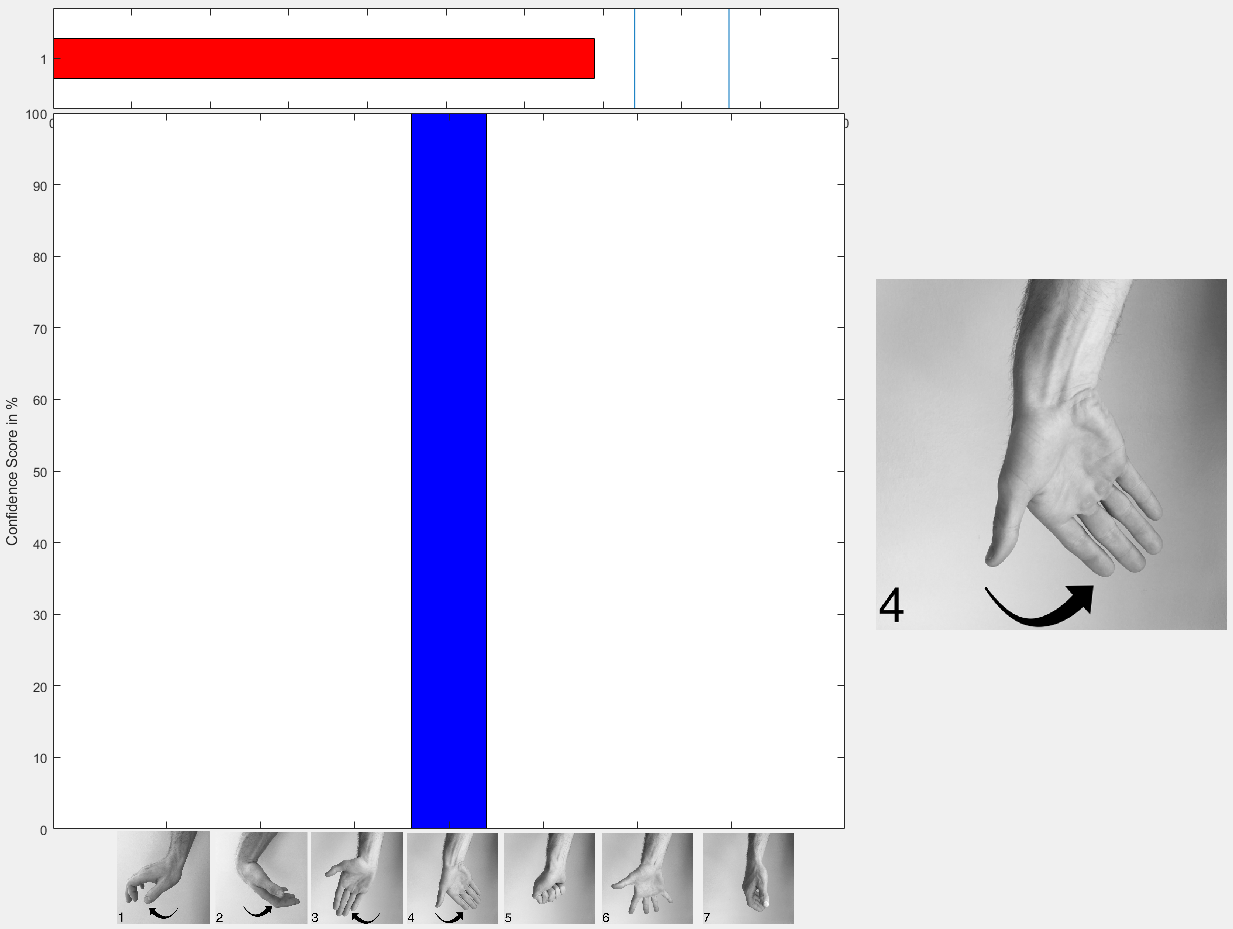
\includegraphics[width=.6\textwidth]{figures/xBackground/usertraincontrolGUI}  
	\caption{Illustration of the user training interface showing the bar plot indicating which movement is being recognized and the text box indicating contraction level.}
	\label{fig:usertraincontrolGUI} 
\end{figure}

\textbf{Performance test}

The purpose of the performance test is to assess the subject's ability to control a prosthesis. Instead of doing a test with a real prosthesis a virtual alternative has been developed for this experiment. The prosthesis is represented as a red circular cursor in a Cartesian coordinate system, which the subject can move as well as expand and shrink in size by performing the trained movement. The following bullets describe which movement corresponds to which action in the coordinate system:

\begin{itemize}
	\item Extension moves the cursor right.
	\item Flexion moves the cursor left.
	\item Radial deviation moves the cursor up.
	\item Ulnar deviation moves the cursor down.
	\item Closed hand shrinks the cursor.
	\item Open hand expands the cursor.
	\item Rest keeps the cursor still.
\end{itemize}

 The performance test consists of a target reaching test, where the subject must reach 16 targets of different sizes and locations. Only one target will be visible at a time. For the subject to reach a target and make a new appear, the subject must center the cursor in the center of the target and expand/shrink the cursor to fit the size of the target. The cursor will appear green, when located at the correct position. The subject must dwell the cursor in a target for 1 seconds for it to be reached. When the cursor has dwelled for 1 second, it will appear blue for 1 second to indicate that the target has been reached. If this is not done within 15 seconds a new target will appear. The aim for the subject is to reach as many target as possible as quickly as possible. The subject is only able to perform one movement at a time, as trained in the user training. Thus, no simultaneously performed movements will be recognized by the control system. The chronology of this step is as follows:

\begin{enumerate}
	\item Reach the visible target.
	\item Repeat step 1 until all targets have been shown.
\end{enumerate}

An illustration of the interface used for the performance test is shown in \figref{fig:perftestGUI}

\begin{figure}[H]                 
	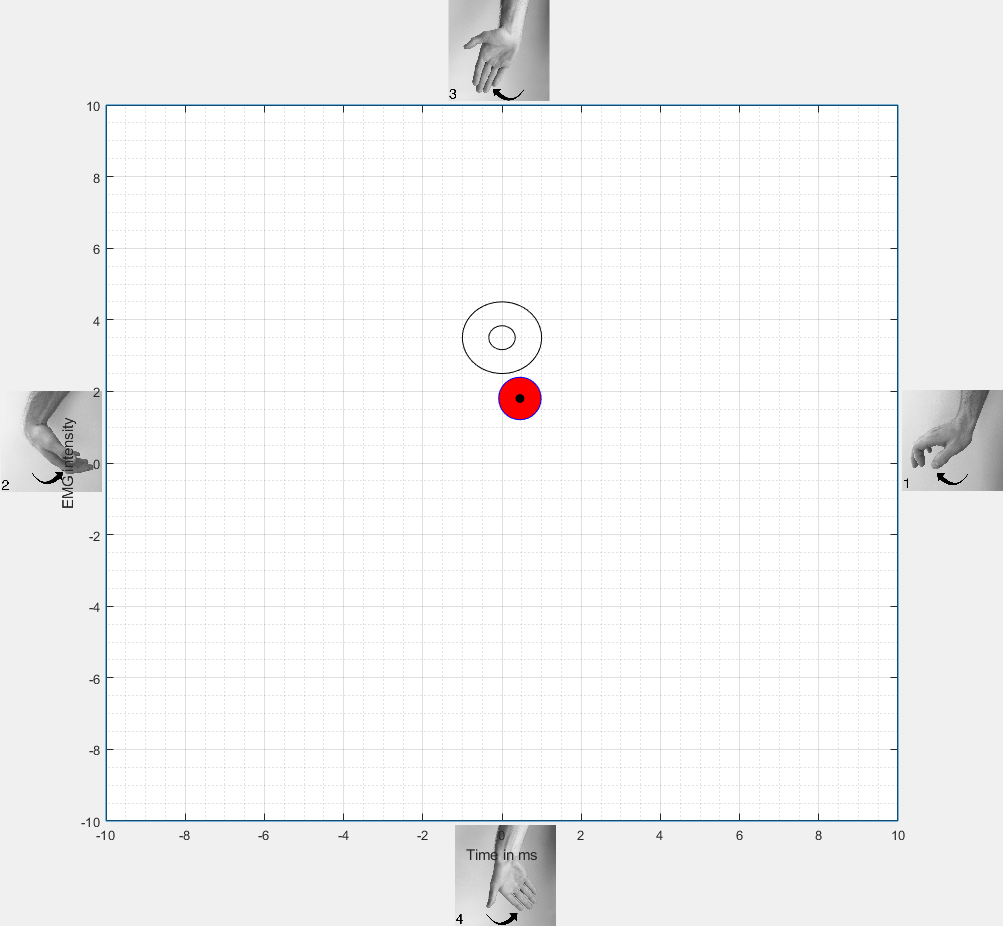
\includegraphics[width=.6\textwidth]{figures/xBackground/perftestGUI}  
	\caption{Illustration of the performance test interface showing a target and the cursor representing the prosthesis output.}
	\label{fig:perftestGUI} 
\end{figure}

\textbf{Movements used in the experiment}

%\begin{figure}[H]                 
%	\includegraphics[width=.6\textwidth]{figures/xBackground/fig:experiment_movements}  
%	\caption{Illustration of the movements used in the experiment. 1: extension, 2: flexion, 3: radial deviation, 4: ulnar deviation, 5: closed hand, 6: open hand and 7: rest}
%	\label{fig:experiment_movements} 
%\end{figure}
%
%Session 1) Data acquisition, user training and performance test and 2) new training data acquisition and performance test. During the training data acquisition EMG data will be recorded from the subject with an EMG-electrode armband (Myo armband from Thalmic Labs) when performing four different wrist movements(flexion, extension, radial deviation and ulnar deviation) as illustrated in \figref{FIGURE}. The data is subsequently used to fit a classification model used in the myoelectric control scheme for the following user training and performance test. Before the performance test the user is given a training period to get familiar with wrist movements used in the performance test. During the performance test the subject will perform a target-reaching task in a cartesian coordinate system of reaching a number of targets using the trained movements by controlling a cursor representing the EMG. Each axis represent one of the four wrist movements, as seen in figure \figref{FIGURE2}, and the open/close hand movements expands/contracts the size of the cursor. The aim for the subject is to reach as many targets as quickly as possible. The subject will perform the target-reaching task twice - one in each session. The subjects are divided into two groups: a test group and a control group. As the study is single-blinded the subject will not be informed which group he/she belongs to.
%
%Chronology of session 1):
%\begin{enumerate}
%	\item Apply MYB on dominant forearm at the thickest part.
%	\item Synchronize MYB by performing wrist extension until three distinct vibrations are felt.
%	\item Perform 15 seconds of maximum voluntary contraction (MVC) of instructed movement. Following the MVC the subject will be given a 30 resting period to avoid fatigue.
%	\item Perform 15 seconds contractions of respectively 20\%, 40\% and 60\% of MVC. During these contractions the subject will control a green marker representing the EMG signal and try to follow a trapezoidal trajectory a precise as possible. The trapezoidal trajectory consists of two five second transition phases and one five second plateau phase as illustrated in figure \figref{FIGURE3}. Between each trial the subject will be given a 15 seconds resting period to avoid muscle fatigue.
%	\item Repeat step 3-4 until training data from all four wrist movements has been recorded.
%	\item The subject will train the seven movements. Each movement will be performed 10 times, where each single movement consists of a five second movement with increased intensity. To improve the precision of movements the subject will receive visual feedback consisting of the probability the movement to belong to based on the classifier. The ideal probability during the training is a 100\% probability of belonging to the trained movement and a 0\% probability of belonging to the remaining movements. 
%	\item The subject will perform a target-reaching task. The subject will control an cursor  in a cartesian coordinate system representing the features extracted from the EMG data, where the length represent the intensity and direction depicts the movement performed. To reach a target the subject must dwell the head of the arrow within the target for 0.5 seconds. If this is achieved the target will disappear. The target will similarly disappear if the subject fails to achieve this within 15 seconds. When an outer target disappears a target centred in origo appears and the subject must reach this before a new outer target appears. This procedure is continued until no more targets are shown. After finishing the performance test the subject will be given a 2 minutes resting period.
%\end{enumerate}
%
%
%Chronology of session 2):
%\begin{enumerate}
%	 \item Perform step 3-5 from session 1.
%	 \item Perform step 7 from session 1. 
%\end{enumerate}
% 









%\chapter{Results}

%\chapter{Discussion}

%\chapter{Conclusion}


	
\begin{multicols}{2}
	
\urlstyle{same}
\printbibliography
%\cleardoublepage
\end{multicols}

%% BILAG
%\begin{appendices}
%	
%\end{appendices}


\end{document}
